

\section{Experiment}
\label{sec:experiments}

We evaluate TS-Memory on long-horizon multivariate forecasting with four research questions (\textbf{RQs}):

\begin{itemize}[leftmargin=*]
    \item \textbf{RQ1:} Can TS-Memory consistently improve various TSFMs across diverse datasets and different backbones? $\rightarrow$ Sec.~\ref{sec:ts_memory_perf_backbones}
    \item \textbf{RQ2:} How does TS-Memory compare with other adaptation strategies in performance and inference latency? $\rightarrow$ Sec.~\ref{sec:comparison_adaptation_baselines}
    \item \textbf{RQ3:} How does TS-Memory perform under backbone scaling and cross-model/cross-dataset transfer? $\rightarrow$ Sec.~\ref{sec:transfer_generality}
    \item \textbf{RQ4:} What are the key design factors of TS-Memory, how do parameter scaling and sensitivity impact its performance, and what qualitative results does it achieve? $\rightarrow$ Sec.~\ref{sec:model_analysis} 
\end{itemize}

% \input{tables/rag vs TS-Memory-simple}

% \begin{table*}[!htbp]
% \begin{center}
% \caption{Long-term forecasting results comparing TS-Memory with online retrieval baselines on ChronosBolt. We use the same protocol in Table~\ref{tab:ts_plugmem_compact}. Full results are in Appendix~\ref{appx:rag-TS-memory} Table~\ref{tab:chronosbolt_base_ablation}.}
% \setlength\tabcolsep{3pt}
% \renewcommand{\arraystretch}{0.80} 
% \scalebox{1}{
% \begin{tabular}{c|ccc|ccc|ccc|ccc}
% \toprule
% \multirow{1}{*}{Method} &
% \multicolumn{3}{c|}{Origin} &
% \multicolumn{3}{c|}{+RAFT} &
% \multicolumn{3}{c|}{+TS RAG} &
% \multicolumn{3}{c}{+TS-Memory} \\
% \midrule
% Metric &
% MSE & MAE & CRPS &
% MSE & MAE & CRPS &
% MSE & MAE & CRPS &
% MSE & MAE & CRPS \\
% \midrule
% ETTh1 & 0.448 & 0.419 & 0.437 & \underline{0.437}\pct{-2.5\%} & \underline{0.418}\pct{-0.2\%} & \underline{0.432}\pct{-1.1\%} & 0.442\pct{-1.3\%} & 0.421\pct{+0.7\%} & 0.440\pct{+0.8\%} & \textbf{0.421}\pct{-6.0\%} & \textbf{0.414}\pct{-1.2\%} & \textbf{0.407}\pct{-6.8\%} \\
% \midrule
% ETTh2 & 0.367 & 0.380 & 0.246 & \underline{0.357}\pct{-2.5\%} & \underline{0.378}\pct{-0.5\%} & \underline{0.243}\pct{-1.0\%} & 0.362\pct{-1.4\%} & 0.385\pct{+1.5\%} & 0.250\pct{+1.6\%} & \textbf{0.354}\pct{-3.4\%} & \textbf{0.375}\pct{-1.1\%} & \textbf{0.238}\pct{-3.1\%} \\
% \midrule
% ETTm1 & 0.421 & 0.383 & 0.409 & \underline{0.397}\pct{-5.5\%} & \underline{0.377}\pct{-1.6\%} & \underline{0.400}\pct{-2.3\%} & 0.406\pct{-3.6\%} & 0.381\pct{-0.4\%} & 0.406\pct{-0.9\%} & \textbf{0.381}\pct{-9.4\%} & \textbf{0.371}\pct{-3.1\%} & \textbf{0.370}\pct{-9.7\%} \\
% \midrule
% ETTm2 & 0.291 & 0.317 & 0.205 & \underline{0.281}\pct{-3.3\%} & \underline{0.315}\pct{-0.9\%} & \underline{0.203}\pct{-1.2\%} & 0.283\pct{-2.6\%} & 0.318\pct{+0.3\%} & 0.205\pct{-0.2\%} & \textbf{0.267}\pct{-8.0\%} & \textbf{0.311}\pct{-2.1\%} & \textbf{0.190}\pct{-7.6\%} \\
% \midrule
% Electricity & 0.159 & 0.244 & 0.239 & \underline{0.156}\pct{-1.5\%} & 0.244\pct{+0.2\%} & 0.240\pct{+0.2\%} & 0.157\pct{-1.4\%} & \underline{0.244}\pct{+0.2\%} & \underline{0.240}\pct{+0.3\%} & \textbf{0.155}\pct{-2.5\%} & \textbf{0.241}\pct{-1.0\%} & \textbf{0.232}\pct{-3.2\%} \\
% \midrule
% Exchange & 0.371 & 0.412 & 0.268 & 0.369\pct{-0.7\%} & 0.408\pct{-0.9\%} & 0.257\pct{-4.2\%} & \underline{0.367}\pct{-1.2\%} & \underline{0.408}\pct{-1.0\%} & \underline{0.253}\pct{-5.6\%} & \textbf{0.365}\pct{-1.8\%} & \textbf{0.406}\pct{-1.5\%} & \textbf{0.250}\pct{-6.9\%} \\
% \midrule
% Traffic & 0.435 & 0.263 & 0.273 & \underline{0.426}\pct{-2.0\%} & \underline{0.261}\pct{-0.8\%} & \underline{0.271}\pct{-0.9\%} & 0.427\pct{-1.9\%} & 0.261\pct{-0.7\%} & 0.271\pct{-0.8\%} & \textbf{0.425}\pct{-2.3\%} & \textbf{0.258}\pct{-1.6\%} & \textbf{0.266}\pct{-2.4\%} \\
% \midrule
% Weather & 0.263 & 0.276 & 0.404 & \underline{0.254}\pct{-3.5\%} & \underline{0.268}\pct{-3.0\%} & \underline{0.390}\pct{-3.5\%} & 0.261\pct{-0.6\%} & 0.279\pct{+1.2\%} & 0.408\pct{+1.0\%} & \textbf{0.239}\pct{-9.1\%} & \textbf{0.267}\pct{-3.5\%} & \textbf{0.370}\pct{-8.4\%} \\
% \bottomrule
% \end{tabular}}
% \label{tab:chronosbolt_base_ablation_compact}
% \end{center}
% \end{table*}

\begin{table*}[!htbp]
\begin{center}
\caption{Long-term forecasting results comparing TS-Memory with online retrieval baselines on ChronosBolt. We use the same protocol as in Table~\ref{tab:ts_plugmem_compact}. Full results are in Table~\ref{tab:chronosbolt_base_ablation} of Appendix~\ref{appx:complete_results} .}
\setlength\tabcolsep{3pt}
\renewcommand{\arraystretch}{0.80} 
\scalebox{0.80}{
\begin{tabular}{c|ccc|ccc|ccc|ccc|ccc}
\toprule
Dataset &
\multicolumn{3}{c|}{Origin} &
\multicolumn{3}{c|}{RAFT} &
\multicolumn{3}{c|}{TS-RAG} &
\multicolumn{3}{c|}{LoRA} &
\multicolumn{3}{c}{TS-Memory} \\
\midrule
Metric &
MSE & MAE & CRPS &
MSE & MAE & CRPS &
MSE & MAE & CRPS &
MSE & MAE & CRPS &
MSE & MAE & CRPS \\
\midrule
ETTh1 & 0.448 & 0.419 & 0.437 & 0.437\pct{-2.5\%} & 0.418\pct{-0.2\%} & 0.432\pct{-1.1\%} & 0.442\pct{-1.3\%} & 0.421\pct{+0.7\%} & 0.440\pct{+0.8\%} & \underline{0.428}\pct{-4.4\%} & \underline{0.416}\pct{-0.6\%} & \underline{0.428}\pct{-2.0\%} & \textbf{0.421}\pct{-6.0\%} & \textbf{0.414}\pct{-1.2\%} & \textbf{0.407}\pct{-6.8\%} \\
\midrule
ETTh2 & 0.367 & 0.380 & 0.246 & 0.357\pct{-2.5\%} & 0.378\pct{-0.5\%} & \underline{0.243}\pct{-1.0\%} & 0.362\pct{-1.4\%} & 0.385\pct{+1.5\%} & 0.250\pct{+1.6\%} & \underline{0.357}\pct{-2.7\%} & \underline{0.377}\pct{-0.6\%} & 0.252\pct{+2.6\%} & \textbf{0.354}\pct{-3.4\%} & \textbf{0.375}\pct{-1.1\%} & \textbf{0.238}\pct{-3.1\%} \\
\midrule
ETTm1 & 0.421 & 0.383 & 0.409 & 0.398\pct{-5.5\%} & 0.377\pct{-1.6\%} & 0.400\pct{-2.3\%} & 0.406\pct{-3.6\%} & 0.381\pct{-0.4\%} & 0.406\pct{-0.9\%} & \underline{0.392}\pct{-6.9\%} & \underline{0.376}\pct{-1.7\%} & \underline{0.397}\pct{-2.9\%} & \textbf{0.381}\pct{-9.4\%} & \textbf{0.371}\pct{-3.1\%} & \textbf{0.370}\pct{-9.7\%} \\
\midrule
ETTm2 & 0.291 & 0.317 & 0.205 & 0.281\pct{-3.3\%} & 0.315\pct{-0.9\%} & 0.203\pct{-1.2\%} & 0.283\pct{-2.6\%} & 0.318\pct{+0.3\%} & 0.205\pct{-0.2\%} & \underline{0.278}\pct{-4.5\%} & \underline{0.314}\pct{-1.2\%} & \underline{0.199}\pct{-3.2\%} & \textbf{0.267}\pct{-8.0\%} & \textbf{0.311}\pct{-2.1\%} & \textbf{0.190}\pct{-7.6\%} \\
\midrule
Electricity & 0.159 & 0.244 & \underline{0.239} & 0.156\pct{-1.5\%} & 0.244\pct{+0.2\%} & 0.240\pct{+0.2\%} & 0.157\pct{-1.4\%} & 0.245\pct{+0.2\%} & 0.240\pct{+0.3\%} & \underline{0.156}\pct{-1.8\%} & \underline{0.244}\pct{-0.1\%} & 0.244\pct{+1.9\%} & \textbf{0.155}\pct{-2.5\%} & \textbf{0.241}\pct{-1.0\%} & \textbf{0.232}\pct{-3.2\%} \\
\midrule
Exchange & 0.371 & 0.412 & 0.268 & 0.369\pct{-0.7\%} & 0.409\pct{-0.9\%} & 0.257\pct{-4.2\%} & 0.367\pct{-1.2\%} & 0.408\pct{-1.0\%} & \underline{0.253}\pct{-5.6\%} & \underline{0.366}\pct{-1.4\%} & \underline{0.407}\pct{-1.2\%} & 0.266\pct{-0.8\%} & \textbf{0.365}\pct{-1.8\%} & \textbf{0.406}\pct{-1.5\%} & \textbf{0.250}\pct{-6.9\%} \\
\midrule
Traffic & 0.435 & 0.263 & 0.273 & 0.426\pct{-2.0\%} & 0.261\pct{-0.8\%} & 0.271\pct{-0.9\%} & 0.427\pct{-1.9\%} & 0.261\pct{-0.7\%} & 0.271\pct{-0.8\%} & \underline{0.425}\pct{-2.2\%} & \underline{0.260}\pct{-1.1\%} & \underline{0.268}\pct{-2.0\%} & \textbf{0.425}\pct{-2.3\%} & \textbf{0.258}\pct{-1.6\%} & \textbf{0.267}\pct{-2.4\%} \\
\midrule
Weather & 0.263 & 0.276 & 0.404 & 0.254\pct{-3.5\%} & \underline{0.268}\pct{-3.0\%} & 0.390\pct{-3.5\%} & 0.262\pct{-0.6\%} & 0.279\pct{+1.2\%} & 0.408\pct{+1.0\%} & \underline{0.247}\pct{-6.1\%} & 0.268\pct{-2.8\%} & \underline{0.378}\pct{-6.4\%} & \textbf{0.239}\pct{-9.1\%} & \textbf{0.267}\pct{-3.5\%} & \textbf{0.370}\pct{-8.4\%} \\
\bottomrule
\end{tabular}}
\label{tab:chronosbolt_base_ablation_compact}
\end{center}

\end{table*}


% \begin{table*}[!htbp]
% \begin{center}
% \caption{Long-term forecasting results comparing TS-Memory with online retrieval baselines on ChronosBolt. We use the same protocol in Table~\ref{tab:ts_plugmem_compact}. Full results are in Appendix~\ref{appx:rag-TS-memory} Table~\ref{tab:chronosbolt_base_ablation}.}
% \setlength\tabcolsep{3pt}
% \renewcommand{\arraystretch}{0.80} 
% \scalebox{1}{
% \begin{tabular}{c|ccc|ccc|ccc|ccc|ccc}
% \toprule
% Dataset &
% \multicolumn{3}{c|}{Origin} &
% \multicolumn{3}{c|}{+RAFT} &
% \multicolumn{3}{c|}{+TS RAG} &
% \multicolumn{3}{c|}{+LoRA} &
% \multicolumn{3}{c}{+TS PlugMem} \\
% \midrule
% Metric &
% MSE & MAE & CRPS &
% MSE & MAE & CRPS &
% MSE & MAE & CRPS &
% MSE & MAE & CRPS &
% MSE & MAE & CRPS \\
% \midrule
% ETTh1 & 0.448 & 0.418 & 0.437 & 0.437 & 0.418 & 0.432 & 0.442 & 0.421 & 0.440 & \underline{0.428} & \underline{0.417} & \underline{0.428} & \textbf{0.421} & \textbf{0.413} & \textbf{0.407} \\
% \midrule
% ETTh2 & 0.367 & 0.380 & 0.246 & \underline{0.357} & \underline{0.378} & \underline{0.243} & 0.362 & 0.385 & 0.250 & 0.359 & 0.380 & 0.252 & \textbf{0.354} & \textbf{0.375} & \textbf{0.238} \\
% \midrule
% ETTm1 & 0.421 & 0.383 & 0.409 & 0.397 & 0.377 & 0.400 & 0.406 & 0.381 & 0.406 & \underline{0.392} & \underline{0.376} & \underline{0.397} & \textbf{0.381} & \textbf{0.371} & \textbf{0.370} \\
% \midrule
% ETTm2 & 0.290 & 0.317 & 0.205 & 0.281 & 0.315 & 0.203 & 0.283 & 0.318 & 0.205 & \underline{0.277} & \underline{0.314} & \underline{0.199} & \textbf{0.267} & \textbf{0.311} & \textbf{0.190} \\
% \midrule
% Electricity & 0.159 & \underline{0.244} & \underline{0.239} & \underline{0.156} & 0.244 & 0.240 & 0.157 & 0.244 & 0.240 & 0.157 & 0.245 & 0.244 & \textbf{0.155} & \textbf{0.241} & \textbf{0.232} \\
% \midrule
% Exchange & 0.371 & 0.412 & 0.268 & 0.369 & 0.408 & 0.257 & 0.367 & 0.408 & \underline{0.253} & \underline{0.366} & \underline{0.407} & 0.266 & \textbf{0.365} & \textbf{0.406} & \textbf{0.250} \\
% \midrule
% Traffic & 0.435 & 0.263 & 0.273 & 0.426 & 0.261 & 0.271 & 0.427 & 0.261 & 0.271 & \underline{0.425} & \underline{0.260} & \underline{0.268} & \textbf{0.425} & \textbf{0.258} & \textbf{0.266} \\
% \midrule
% Weather & 0.263 & 0.276 & 0.404 & 0.254 & \underline{0.268} & 0.390 & 0.261 & 0.279 & 0.408 & \underline{0.247} & 0.268 & \underline{0.378} & \textbf{0.239} & \textbf{0.267} & \textbf{0.370} \\
% \bottomrule
% \end{tabular}}
% \label{tab:chronosbolt_base_ablation_compact}
% \end{center}
% \end{table*}
\begin{table*}[!htbp]
\begin{center}
\caption{Inference latency comparison (ms/query) for Origin, online retrieval baselines, LoRA, and TS-Memory on ChronosBolt. We report retrieval time (Retr), forward time (Fwd), total time (Total), and retrieval fraction (Frac), following the same protocol as Table~\ref{tab:ts_plugmem_compact}. Full results are in  Table~\ref{tab:chronosbolt_time_latency} of Appendix~\ref{appx:complete_results}.}

\renewcommand{\arraystretch}{0.80} 
\setlength\tabcolsep{2pt}
\scalebox{0.83}{
\begin{tabular}{c|cccc|cccc|cccc|cccc|cccc}
\toprule
\multirow{1}{*}{Method} &
\multicolumn{4}{c|}{Origin} &
\multicolumn{4}{c|}{RAFT} &
\multicolumn{4}{c|}{TS-RAG} &
\multicolumn{4}{c|}{LoRA} &
\multicolumn{4}{c}{TS-Memory} \\
\midrule
\multirow{1}{*}{Metric}
& Retr & Fwd & Total & Frac &
Retr & Fwd & Total & Frac &
Retr & Fwd & Total & Frac &
Retr & Fwd & Total & Frac &
Retr & Fwd & Total & Frac \\
\midrule
ETTh1
& 0 & 3.53 & 3.53 & 0\%
& 0.84 & 3.84\pct{+8.8\%} & 4.68\pct{+32.6\%} & 20.0\%
& 3.53 & \underline{3.80}\pct{+7.8\%} & 7.33\pct{+107.9\%} & 51.1\%
& \underline{0} & 4.28\pct{+21.4\%} & \underline{4.28}\pct{+21.4\%} & \underline{0\%}
& \textbf{0} & \textbf{3.69}\pct{+4.7\%} & \textbf{3.69}\pct{+4.7\%} & \textbf{0\%} \\
\midrule
ETTh2
& 0 & 3.52 & 3.52 & 0\%
& 0.84 & \underline{3.82}\pct{+8.4\%} & 4.65\pct{+32.1\%} & 19.7\%
& 3.50 & 3.83\pct{+8.7\%} & 7.33\pct{+108.2\%} & 50.6\%
& \underline{0} & 4.29\pct{+21.7\%} & \underline{4.29}\pct{+21.7\%} & \underline{0\%}
& \textbf{0} & \textbf{3.66}\pct{+4.0\%} & \textbf{3.66}\pct{+4.0\%} & \textbf{0\%} \\
\midrule
ETTm1
& 0 & 3.52 & 3.52 & 0\%
& 2.62 & 3.79\pct{+7.5\%} & 6.41\pct{+81.9\%} & 43.9\%
& 6.46 & \underline{3.78}\pct{+7.4\%} & 10.24\pct{+190.6\%} & 65.7\%
& \underline{0} & 4.24\pct{+20.4\%} & \underline{4.24}\pct{+20.4\%} & \underline{0\%}
& \textbf{0} & \textbf{3.67}\pct{+4.1\%} & \textbf{3.67}\pct{+4.1\%} & \textbf{0\%} \\
\midrule
ETTm2
& 0 & 3.52 & 3.52 & 0\%
& 2.52 & \underline{3.79}\pct{+7.5\%} & 6.30\pct{+79.0\%} & 43.4\%
& 6.44 & 3.80\pct{+7.8\%} & 10.23\pct{+190.5\%} & 65.6\%
& \underline{0} & 4.24\pct{+20.4\%} & \underline{4.24}\pct{+20.4\%} & \underline{0\%}
& \textbf{0} & \textbf{3.66}\pct{+3.9\%} & \textbf{3.66}\pct{+3.9\%} & \textbf{0\%} \\
\midrule
Electricity
& 0 & 3.51 & 3.51 & 0\%
& 1.49 & \underline{3.79}\pct{+8.0\%} & 5.28\pct{+50.4\%} & 31.2\%
& 4.62 & 3.79\pct{+8.2\%} & 8.41\pct{+139.7\%} & 57.9\%
& \underline{0} & 3.89\pct{+11.0\%} & \underline{3.89}\pct{+11.0\%} & \underline{0\%}
& \textbf{0} & \textbf{3.64}\pct{+3.8\%} & \textbf{3.64}\pct{+3.8\%} & \textbf{0\%} \\
\midrule
Exchange
& 0 & 3.53 & 3.53 & 0\%
& 0.51 & \underline{3.79}\pct{+7.5\%} & 4.30\pct{+21.9\%} & 13.3\%
& 3.07 & 3.79\pct{+7.6\%} & 6.87\pct{+94.7\%} & 47.7\%
& \underline{0} & 4.29\pct{+21.7\%} & \underline{4.29}\pct{+21.7\%} & \underline{0\%}
& \textbf{0} & \textbf{3.66}\pct{+3.8\%} & \textbf{3.66}\pct{+3.8\%} & \textbf{0\%} \\
\midrule
Traffic
& 0 & 3.51 & 3.51 & 0\%
& 1.04 & \underline{3.79}\pct{+8.0\%} & 4.82\pct{+37.5\%} & 23.8\%
& 3.90 & 3.79\pct{+8.1\%} & 7.69\pct{+119.2\%} & 53.7\%
& \underline{0} & 3.88\pct{+10.7\%} & \underline{3.88}\pct{+10.7\%} & \underline{0\%}
& \textbf{0} & \textbf{3.64}\pct{+3.8\%} & \textbf{3.64}\pct{+3.8\%} & \textbf{0\%} \\
\midrule
Weather
& 0 & 3.52 & 3.52 & 0\%
& 2.71 & \underline{3.79}\pct{+7.7\%} & 6.49\pct{+84.6\%} & 44.7\%
& 6.67 & 3.79\pct{+7.8\%} & 10.47\pct{+197.6\%} & 66.4\%
& \underline{0} & 3.96\pct{+12.6\%} & \underline{3.96}\pct{+12.6\%} & \underline{0\%}
& \textbf{0} & \textbf{3.65}\pct{+3.9\%} & \textbf{3.65}\pct{+3.9\%} & \textbf{0\%} \\
\bottomrule
\end{tabular}}
\label{tab:chronosbolt_time_latency_compact}

\end{center}
\end{table*}



\subsection{Experimental Setup}

\noindent\textbf{Datasets \& Evaluation Metrics.} We experiment on eight widely used multivariate long-term forecasting benchmarks (ETTh1/2, ETTm1/2, Electricity, Exchange-rate, Traffic, Weather)~\cite{zhou2021informer,lai2018modeling}. Following the standard long-horizon protocol, we evaluate across multiple forecasting horizons and report the average performance to characterize overall long-range forecasting ability~\cite{wu2023timesnet}. For point forecasting, we report \textit{MSE} and \textit{MAE}~\cite{hyndman2006another}; for probabilistic forecasting, we additionally present \textit{CRPS} to assess prediction quality~\cite{gneiting2007strictly}.

\noindent\textbf{Baselines \& Backbones.} 
We adopt four representative TSFMs: \textit{ChronosBolt}~\cite{ansari2024chronos}, \textit{Chronos2}~\cite{ansari2025chronos}, \textit{Sundial}~\cite{liu2025sundial} and \textit{TimesFM}~\cite{das2024decoder}, with backbone parameters frozen unless specified otherwise. 
We compare against three baselines: 
\textit{(1)} \textit{Origin}, the zero-shot deployment of frozen backbones; 
\textit{(2)} Online retrieval augmentation baselines (\textit{RAFT}~\cite{han2025retrieval}, \textit{TS-RAG}~
\cite{ning2025ts}), which perform test-time $k$NN retrieval from a leakage-safe datastore and fuse retrieved futures for forecasting; 
\textit{(3)} The parameter-efficient fine-tuning baseline \textit{LoRA}, which injects low-rank adapters into attention projection layers and only trains the adapters, with trainable parameters matched to PlugMem.

\noindent\textbf{Implementation Details.} Following prior work~\cite{wu2023timesnet}, we use prediction horizons $H \in \{96, 192, 336, 720\}$ and a fixed look-back window of $L = 512$. All models are optimized via Adam~\cite{kingma2014adam}. For baseline methods on backbone models, we strictly adhere to their original hyperparameter settings to ensure fair comparison. All experiments are implemented in PyTorch and run on NVIDIA A800 80GB GPUs. Additional details are provided in Appendix~\ref{appx:experiment_details}.




\subsection{TS-Memory Performance Across Backbones}
\label{sec:ts_memory_perf_backbones}

Table~\ref{tab:ts_plugmem_compact} presents long-horizon forecasting results for TS-Memory deployed on four frozen TSFM backbones across eight benchmarks. TS-Memory enhances all backbones on every dataset, confirming that retrieval-driven gains can be distilled into a compact memory module without backbone parameter update. Averaged across all dataset–backbone pairs, TS-Memory reduces MSE by 5.8\% and MAE by 2.1\%, with peak reductions of 16.0\% (MSE) and 6.0\% (MAE). Gains are most pronounced on benchmarks with severe distribution shifts and rich temporal structures (e.g., Weather and ETT minute-level datasets), where double-digit MSE reductions are common, demonstrating improved robustness to long-horizon error accumulation. For regular benchmarks (e.g., Electricity), improvements are modest yet consistent. It matches the desired plug-and-play adapter behavior: substantial gains for poorly performing zero-shot backbones, and stability for well-aligned ones. Consistent MAE reductions further confirm broad error mitigation across time steps and variables, rather than sporadic gains in isolated cases.

\noindent\textbf{Pretraining-overlap check.}
Our retrieval-leakage-safe construction rules out test-window leakage for the offline teacher and online retrieval baselines, but does not assume fully auditable TSFM pretraining corpora. We therefore exclude confirmable backbone--dataset overlap pairs: TimesFM on Electricity, Traffic, and Weather; Sundial on Traffic; and Chronos2 on Electricity. On the $27$ pairs, TS-Memory reduces MSE by $6.22\%$ and MAE by $2.18\%$, slightly stronger than the full $32$-pair reductions of $5.8\%$ and $2.1\%$. This suggests our gains are not driven by known pretraining overlap.

\begin{table*}[!htbp]
\begin{center}
\caption{Scaling study of TS-Memory across ChronosBolt model sizes. We use the same protocol as in Table~\ref{tab:ts_plugmem_compact}. Full results are in 
Table~\ref{tab:chronosbolt_ts_plugmem_full} of Appendix~\ref{appx:complete_results}.}

\begin{small}
\setlength\tabcolsep{3pt}
\renewcommand{\arraystretch}{0.85} 
\scalebox{0.9}{
\begin{tabular}{c|cc|cc|cc|cc|cc|cc|cc|cc}
\toprule
\multirow{1}{*}{Model} &
\multicolumn{4}{c|}{ChronosBolt Base (205M)} &
\multicolumn{4}{c|}{ChronosBolt Small (48M)} &
\multicolumn{4}{c|}{ChronosBolt Mini (21M)} &
\multicolumn{4}{c}{ChronosBolt Tiny (9M)} \\
\cmidrule{1-17}
\multirow{1}{*}{Dataset} &
\multicolumn{2}{c|}{Origin} & \multicolumn{2}{c|}{TS-Memory} &
\multicolumn{2}{c|}{Origin} & \multicolumn{2}{c|}{TS-Memory} &
\multicolumn{2}{c|}{Origin} & \multicolumn{2}{c|}{TS-Memory} &
\multicolumn{2}{c|}{Origin} & \multicolumn{2}{c}{TS-Memory} \\
\midrule
Metric &
MSE & MAE & MSE & MAE &
MSE & MAE & MSE & MAE &
MSE & MAE & MSE & MAE &
MSE & MAE & MSE & MAE \\
\midrule
ETTh1 & \underline{0.448} & \underline{0.419} & \textbf{0.421}\pct{-6.0\%} & \textbf{0.414}\pct{-1.2\%} & \underline{0.463} & \underline{0.422} & \textbf{0.437}\pct{-5.5\%} & \textbf{0.417}\pct{-1.2\%} & \underline{0.445} & \underline{0.421} & \textbf{0.424}\pct{-4.8\%} & \textbf{0.417}\pct{-1.0\%} & \underline{0.447} & \underline{0.422} & \textbf{0.427}\pct{-4.6\%} & \textbf{0.418}\pct{-1.0\%} \\
\midrule
ETTh2 & \underline{0.367} & \underline{0.380} & \textbf{0.354}\pct{-3.4\%} & \textbf{0.375}\pct{-1.1\%} & \underline{0.362} & \underline{0.382} & \textbf{0.357}\pct{-1.5\%} & \textbf{0.379}\pct{-0.7\%} & \underline{0.370} & \underline{0.384} & \textbf{0.358}\pct{-3.2\%} & \textbf{0.380}\pct{-1.0\%} & \underline{0.367} & \underline{0.385} & \textbf{0.361}\pct{-1.7\%} & \textbf{0.383}\pct{-0.7\%} \\
\midrule
ETTm1 & \underline{0.421} & \underline{0.383} & \textbf{0.381}\pct{-9.4\%} & \textbf{0.371}\pct{-3.1\%} & \underline{0.420} & \underline{0.385} & \textbf{0.377}\pct{-10.3\%} & \textbf{0.373}\pct{-3.1\%} & \underline{0.417} & \underline{0.385} & \textbf{0.374}\pct{-10.3\%} & \textbf{0.372}\pct{-3.2\%} & \underline{0.407} & \underline{0.385} & \textbf{0.373}\pct{-8.4\%} & \textbf{0.375}\pct{-2.7\%} \\
\midrule
ETTm2 & \underline{0.291} & \underline{0.317} & \textbf{0.267}\pct{-8.0\%} & \textbf{0.311}\pct{-2.1\%} & \underline{0.284} & \underline{0.317} & \textbf{0.266}\pct{-6.4\%} & \textbf{0.311}\pct{-1.7\%} & \underline{0.290} & \underline{0.319} & \textbf{0.266}\pct{-8.2\%} & \textbf{0.312}\pct{-2.2\%} & \underline{0.284} & \underline{0.317} & \textbf{0.264}\pct{-7.2\%} & \textbf{0.312}\pct{-1.8\%} \\
\midrule
Electricity & \underline{0.159} & \underline{0.244} & \textbf{0.155}\pct{-2.5\%} & \textbf{0.241}\pct{-1.0\%} & \underline{0.163} & \underline{0.249} & \textbf{0.159}\pct{-2.5\%} & \textbf{0.246}\pct{-1.1\%} & \underline{0.167} & \underline{0.253} & \textbf{0.163}\pct{-2.5\%} & \textbf{0.251}\pct{-0.8\%} & \underline{0.172} & \underline{0.259} & \textbf{0.166}\pct{-3.1\%} & \textbf{0.256}\pct{-1.2\%} \\
\midrule
Traffic & \underline{0.435} & \underline{0.263} & \textbf{0.425}\pct{-2.3\%} & \textbf{0.258}\pct{-1.6\%} & \underline{0.412} & \underline{0.264} & \textbf{0.408}\pct{-1.1\%} & \textbf{0.260}\pct{-1.4\%} & \underline{0.417} & \underline{0.269} & \textbf{0.411}\pct{-1.2\%} & \textbf{0.265}\pct{-1.3\%} & \underline{0.419} & \underline{0.276} & \textbf{0.414}\pct{-1.2\%} & \textbf{0.271}\pct{-2.1\%} \\
\midrule
Weather & \underline{0.263} & \underline{0.276} & \textbf{0.239}\pct{-9.1\%} & \textbf{0.267}\pct{-3.5\%} & \underline{0.256} & \underline{0.270} & \textbf{0.239}\pct{-6.5\%} & \textbf{0.266}\pct{-1.8\%} & \underline{0.268} & \underline{0.283} & \textbf{0.240}\pct{-10.6\%} & \textbf{0.273}\pct{-3.4\%} & \underline{0.271} & \underline{0.286} & \textbf{0.239}\pct{-11.7\%} & \textbf{0.275}\pct{-3.8\%} \\
\bottomrule
\end{tabular}}
\end{small}
\label{tab:chronosbolt_ts_memory_compact}
\vspace{-0.5em}
\end{center}
\end{table*}
% % Requires:
% % \usepackage{booktabs,multirow}
% % \usepackage{caption}

% \begin{table*}[h!]
% \begin{center}
% \caption{Cross-model TS-Memory transfer evaluation. Values in parentheses denote relative change (\%) compared to Origin.}
% \begin{small}
% \renewcommand{\arraystretch}{0.80} 
% \setlength\tabcolsep{2pt}
% \resizebox{\textwidth}{!}{%
% \begin{tabular}{l|cc|cc|cc|cc|cc|cc||cc|cc|cc|cc|cc|cc}
% \toprule
% \multirow{2}{*}{Dataset} & \multicolumn{12}{c||}{Chronos2-PlugMem} & \multicolumn{12}{c}{Sundial-PlugMem} \\
% \cmidrule{2-25}
%  &
% \multicolumn{4}{c|}{ChronosBolt (base)} &
% \multicolumn{4}{c|}{Sundial (base)} &
% \multicolumn{4}{c||}{TimesFM (base)} &
% \multicolumn{4}{c|}{ChronosBolt (base)} &
% \multicolumn{4}{c|}{Chronos2 (base)} &
% \multicolumn{4}{c}{TimesFM (base)} \\
% \midrule
% Metric &
% \multicolumn{2}{c|}{Origin} & \multicolumn{2}{c|}{+TS Mem} &
% \multicolumn{2}{c|}{Origin} & \multicolumn{2}{c|}{+TS Mem} &
% \multicolumn{2}{c|}{Origin} & \multicolumn{2}{c||}{+TS Mem} &
% \multicolumn{2}{c|}{Origin} & \multicolumn{2}{c|}{+TS Mem} &
% \multicolumn{2}{c|}{Origin} & \multicolumn{2}{c|}{+TS Mem} &
% \multicolumn{2}{c|}{Origin} & \multicolumn{2}{c}{+TS Mem} \\
% \midrule
%  &
% MSE & MAE & MSE & MAE &
% MSE & MAE & MSE & MAE &
% MSE & MAE & MSE & MAE &
% MSE & MAE & MSE & MAE &
% MSE & MAE & MSE & MAE &
% MSE & MAE & MSE & MAE \\
% \midrule

% ETTh1 & 0.448 & 0.419 & \textbf{0.420}{\scriptsize(-6.2\%)} & \textbf{0.416}{\scriptsize(-0.6\%)} & 0.400 & 0.412 & \textbf{0.395}{\scriptsize(-1.1\%)} & \textbf{0.410}{\scriptsize(-0.5\%)} & 0.479 & 0.442 & \textbf{0.436}{\scriptsize(-9.1\%)} & \textbf{0.430}{\scriptsize(-2.8\%)} & 0.448 & 0.419 & \textbf{0.409}{\scriptsize(-8.6\%)} & \textbf{0.416}{\scriptsize(-0.7\%)} & 0.442 & 0.412 & \textbf{0.409}{\scriptsize(-7.6\%)} & 0.412{\scriptsize(+0.2\%)} & 0.479 & 0.442 & \textbf{0.424}{\scriptsize(-11.5\%)} & \textbf{0.427}{\scriptsize(-3.6\%)} \\
% \midrule
% ETTh2 & 0.366 & 0.380 & \textbf{0.342}{\scriptsize(-6.6\%)} & 0.383{\scriptsize(+0.9\%)} & 0.344 & 0.380 & \textbf{0.338}{\scriptsize(-1.6\%)} & \textbf{0.379}{\scriptsize(-0.1\%)} & 0.402 & 0.409 & \textbf{0.358}{\scriptsize(-10.9\%)} & \textbf{0.402}{\scriptsize(-1.9\%)} & 0.366 & 0.380 & \textbf{0.339}{\scriptsize(-7.4\%)} & 0.382{\scriptsize(+0.6\%)} & 0.376 & 0.383 & \textbf{0.347}{\scriptsize(-7.6\%)} & 0.384{\scriptsize(+0.1\%)} & 0.402 & 0.409 & \textbf{0.356}{\scriptsize(-11.4\%)} & \textbf{0.399}{\scriptsize(-2.5\%)} \\
% \midrule
% ETTm1 & 0.421 & 0.383 & \textbf{0.375}{\scriptsize(-10.9\%)} & \textbf{0.375}{\scriptsize(-2.0\%)} & 0.369 & 0.369 & \textbf{0.356}{\scriptsize(-3.5\%)} & \textbf{0.366}{\scriptsize(-0.8\%)} & 0.429 & 0.416 & \textbf{0.375}{\scriptsize(-12.5\%)} & \textbf{0.390}{\scriptsize(-6.2\%)} & 0.421 & 0.383 & \textbf{0.367}{\scriptsize(-12.8\%)} & \textbf{0.375}{\scriptsize(-2.0\%)} & 0.433 & 0.381 & \textbf{0.370}{\scriptsize(-14.6\%)} & \textbf{0.378}{\scriptsize(-0.7\%)} & 0.429 & 0.416 & \textbf{0.372}{\scriptsize(-13.2\%)} & \textbf{0.390}{\scriptsize(-6.2\%)} \\
% \midrule
% ETTm2 & 0.290 & 0.317 & \textbf{0.262}{\scriptsize(-9.8\%)} & \textbf{0.314}{\scriptsize(-1.1\%)} & 0.276 & 0.317 & \textbf{0.262}{\scriptsize(-4.9\%)} & \textbf{0.314}{\scriptsize(-1.1\%)} & 0.332 & 0.341 & \textbf{0.267}{\scriptsize(-19.4\%)} & \textbf{0.322}{\scriptsize(-5.6\%)} & 0.290 & 0.317 & \textbf{0.265}{\scriptsize(-8.7\%)} & \textbf{0.314}{\scriptsize(-1.2\%)} & 0.295 & 0.315 & \textbf{0.264}{\scriptsize(-10.4\%)} & \textbf{0.313}{\scriptsize(-0.8\%)} & 0.332 & 0.341 & \textbf{0.273}{\scriptsize(-17.7\%)} & \textbf{0.325}{\scriptsize(-4.8\%)} \\
% \midrule
% Electricity & 0.159 & 0.244 & \textbf{0.154}{\scriptsize(-3.0\%)} & \textbf{0.242}{\scriptsize(-0.9\%)} & 0.148 & 0.242 & \textbf{0.144}{\scriptsize(-2.6\%)} & \textbf{0.238}{\scriptsize(-1.5\%)} & 0.154 & 0.244 & \textbf{0.151}{\scriptsize(-2.0\%)} & \textbf{0.242}{\scriptsize(-0.8\%)} & 0.159 & 0.244 & \textbf{0.154}{\scriptsize(-2.9\%)} & \textbf{0.243}{\scriptsize(-0.5\%)} & 0.163 & 0.244 & \textbf{0.157}{\scriptsize(-3.4\%)} & \textbf{0.242}{\scriptsize(-0.7\%)} & 0.154 & 0.244 & \textbf{0.151}{\scriptsize(-2.0\%)} & \textbf{0.243}{\scriptsize(-0.5\%)} \\
% \midrule
% Exchange & 0.371 & 0.412 & \textbf{0.355}{\scriptsize(-4.4\%)} & \textbf{0.405}{\scriptsize(-1.7\%)} & 0.553 & 0.494 & \textbf{0.408}{\scriptsize(-26.3\%)} & \textbf{0.444}{\scriptsize(-9.9\%)} & 0.433 & 0.446 & \textbf{0.383}{\scriptsize(-11.5\%)} & \textbf{0.427}{\scriptsize(-4.1\%)} & 0.371 & 0.412 & \textbf{0.365}{\scriptsize(-1.6\%)} & \textbf{0.407}{\scriptsize(-1.1\%)} & 0.399 & 0.421 & \textbf{0.392}{\scriptsize(-1.7\%)} & \textbf{0.417}{\scriptsize(-0.9\%)} & 0.433 & 0.446 & \textbf{0.420}{\scriptsize(-3.1\%)} & \textbf{0.438}{\scriptsize(-1.8\%)} \\
% \midrule
% Traffic & 0.435 & 0.263 & \textbf{0.417}{\scriptsize(-4.1\%)} & \textbf{0.260}{\scriptsize(-0.9\%)} & 0.461 & 0.286 & \textbf{0.427}{\scriptsize(-7.3\%)} & \textbf{0.275}{\scriptsize(-4.0\%)} & 0.370 & 0.244 & \textbf{0.366}{\scriptsize(-0.9\%)} & \textbf{0.243}{\scriptsize(-0.4\%)} & 0.435 & 0.263 & \textbf{0.418}{\scriptsize(-3.9\%)} & \textbf{0.261}{\scriptsize(-0.8\%)} & 0.394 & 0.237 & \textbf{0.388}{\scriptsize(-1.7\%)} & 0.240{\scriptsize(+1.3\%)} & 0.370 & 0.244 & \textbf{0.367}{\scriptsize(-0.7\%)} & \textbf{0.243}{\scriptsize(-0.2\%)} \\
% \midrule
% Weather & 0.263 & 0.276 & \textbf{0.235}{\scriptsize(-10.8\%)} & \textbf{0.269}{\scriptsize(-2.7\%)} & 0.244 & 0.269 & \textbf{0.235}{\scriptsize(-3.5\%)} & \textbf{0.269}{\scriptsize(-0.3\%)} & 0.222 & 0.237 & \textbf{0.198}{\scriptsize(-10.7\%)} & \textbf{0.232}{\scriptsize(-2.4\%)} & 0.263 & 0.276 & \textbf{0.235}{\scriptsize(-10.5\%)} & \textbf{0.273}{\scriptsize(-1.2\%)} & 0.274 & 0.267 & \textbf{0.233}{\scriptsize(-14.7\%)} & 0.268{\scriptsize(+0.5\%)} & 0.222 & 0.237 & \textbf{0.198}{\scriptsize(-10.5\%)} & \textbf{0.233}{\scriptsize(-1.8\%)} \\

% \bottomrule
% \end{tabular}}
% \end{small}
% \label{tab:plugmem_merged_compact}
% \end{center}
% \end{table*}


% Requires:
% \usepackage{booktabs,multirow}
% \usepackage{caption}

% Requires:
% \usepackage{booktabs,multirow}
% \usepackage{caption}

% \begin{table*}[h!]
% \begin{center}
% \caption{Cross-model transfer results of TS-Memory across retrieval teachers and frozen TSFM backbones. We use the same protocol in Table~\ref{tab:ts_plugmem_compact}. Full results are in Appendix~\ref{appx:rag-TS-memory} Table~\ref{tab:plugmem_merged}.
% }
% \begin{small}
% \renewcommand{\arraystretch}{0.80} 
% \setlength\tabcolsep{2pt}
% \resizebox{\textwidth}{!}{%
% \begin{tabular}{c|cc|cc|cc|cc|cc|cc||cc|cc|cc|cc|cc|cc}
% \toprule
% \multirow{2}{*}{Model} & \multicolumn{12}{c||}{Chronos2-PlugMem} & \multicolumn{12}{c}{Sundial-PlugMem} \\
% \cmidrule{2-25}
%  &
% \multicolumn{4}{c|}{ChronosBolt (base)} &
% \multicolumn{4}{c|}{Sundial (base)} &
% \multicolumn{4}{c||}{TimesFM (base)} &
% \multicolumn{4}{c|}{ChronosBolt (base)} &
% \multicolumn{4}{c|}{Chronos2 (base)} &
% \multicolumn{4}{c}{TimesFM (base)} \\
% \midrule
% Dataset &
% \multicolumn{2}{c|}{Origin} & \multicolumn{2}{c|}{+TS Mem} &
% \multicolumn{2}{c|}{Origin} & \multicolumn{2}{c|}{+TS Mem} &
% \multicolumn{2}{c|}{Origin} & \multicolumn{2}{c||}{+TS Mem} &
% \multicolumn{2}{c|}{Origin} & \multicolumn{2}{c|}{+TS Mem} &
% \multicolumn{2}{c|}{Origin} & \multicolumn{2}{c|}{+TS Mem} &
% \multicolumn{2}{c|}{Origin} & \multicolumn{2}{c}{+TS Mem} \\
% \midrule
% Metric &
% MSE & MAE & MSE & MAE &
% MSE & MAE & MSE & MAE &
% MSE & MAE & MSE & MAE &
% MSE & MAE & MSE & MAE &
% MSE & MAE & MSE & MAE &
% MSE & MAE & MSE & MAE \\
% \midrule

% ETTh1 & 0.448 & 0.419 & \textbf{0.420} & \textbf{0.416} & 0.400 & 0.412 & \textbf{0.395} & \textbf{0.410} & 0.479 & 0.442 & \textbf{0.436} & \textbf{0.430} & 0.448 & 0.419 & \textbf{0.409} & \textbf{0.416} & 0.442 & \textbf{0.412} & \textbf{0.409} & 0.412 & 0.479 & 0.442 & \textbf{0.424} & \textbf{0.427} \\
% \midrule
% ETTh2 & 0.366 & \textbf{0.380} & \textbf{0.342} & 0.383 & 0.344 & 0.380 & \textbf{0.338} & \textbf{0.379} & 0.402 & 0.409 & \textbf{0.358} & \textbf{0.402} & 0.366 & \textbf{0.380} & \textbf{0.339} & 0.382 & 0.376 & \textbf{0.383} & \textbf{0.347} & 0.384 & 0.402 & 0.409 & \textbf{0.356} & \textbf{0.399} \\
% \midrule
% ETTm1 & 0.421 & 0.383 & \textbf{0.375} & \textbf{0.375} & 0.369 & 0.369 & \textbf{0.356} & \textbf{0.366} & 0.429 & 0.416 & \textbf{0.375} & \textbf{0.390} & 0.421 & 0.383 & \textbf{0.367} & \textbf{0.375} & 0.433 & 0.381 & \textbf{0.370} & \textbf{0.378} & 0.429 & 0.416 & \textbf{0.372} & \textbf{0.390} \\
% \midrule
% ETTm2 & 0.290 & 0.317 & \textbf{0.262} & \textbf{0.314} & 0.276 & 0.317 & \textbf{0.262} & \textbf{0.314} & 0.332 & 0.341 & \textbf{0.267} & \textbf{0.322} & 0.290 & 0.317 & \textbf{0.265} & \textbf{0.314} & 0.295 & 0.315 & \textbf{0.264} & \textbf{0.313} & 0.332 & 0.341 & \textbf{0.273} & \textbf{0.325} \\
% \midrule
% Electricity & 0.159 & 0.244 & \textbf{0.154} & \textbf{0.242} & 0.148 & 0.242 & \textbf{0.144} & \textbf{0.238} & 0.154 & 0.244 & \textbf{0.151} & \textbf{0.242} & 0.159 & 0.244 & \textbf{0.154} & \textbf{0.243} & 0.163 & 0.244 & \textbf{0.157} & \textbf{0.242} & 0.154 & 0.244 & \textbf{0.151} & \textbf{0.243} \\
% \midrule
% Exchange & 0.371 & 0.412 & \textbf{0.355} & \textbf{0.405} & 0.553 & 0.494 & \textbf{0.408} & \textbf{0.444} & 0.433 & 0.446 & \textbf{0.383} & \textbf{0.427} & 0.371 & 0.412 & \textbf{0.365} & \textbf{0.407} & 0.399 & 0.421 & \textbf{0.392} & \textbf{0.417} & 0.433 & 0.446 & \textbf{0.420} & \textbf{0.438} \\
% \midrule
% Traffic & 0.435 & 0.263 & \textbf{0.417} & \textbf{0.260} & 0.461 & 0.286 & \textbf{0.427} & \textbf{0.275} & 0.370 & 0.244 & \textbf{0.366} & \textbf{0.243} & 0.435 & 0.263 & \textbf{0.418} & \textbf{0.261} & 0.394 & \textbf{0.237} & \textbf{0.388} & 0.240 & 0.370 & 0.244 & \textbf{0.367} & \textbf{0.243} \\
% \midrule
% Weather & 0.263 & 0.276 & \textbf{0.235} & \textbf{0.269} & 0.244 & 0.269 & \textbf{0.235} & \textbf{0.269} & 0.222 & 0.237 & \textbf{0.198} & \textbf{0.232} & 0.263 & 0.276 & \textbf{0.235} & \textbf{0.273} & 0.274 & \textbf{0.267} & \textbf{0.233} & 0.268 & 0.222 & 0.237 & \textbf{0.198} & \textbf{0.233} \\

% \bottomrule
% \end{tabular}}
% \end{small}
% \label{tab:plugmem_merged_compact}
% \end{center}
% \end{table*}

% Requires:
% \usepackage{booktabs,multirow}
% \usepackage{caption}

\begin{table*}[!htbp]
\begin{center}
\caption{Cross-model transfer results of TS-Memory across retrieval teachers and frozen TSFM backbones. We use the same protocol as in Table~\ref{tab:ts_plugmem_compact}. Full results are in Table~\ref{tab:plugmem_merged} of Appendix~\ref{appx:complete_results}.
}

\begin{small}
\renewcommand{\arraystretch}{0.80} 
\setlength\tabcolsep{2pt}
\resizebox{\textwidth}{!}{%
\begin{tabular}{c|cc|cc|cc|cc|cc|cc||cc|cc|cc|cc|cc|cc}
\toprule
\multirow{2}{*}{Model} & \multicolumn{12}{c||}{Chronos2-PlugMem} & \multicolumn{12}{c}{Sundial-PlugMem} \\
\cmidrule{2-25}
 &
\multicolumn{4}{c|}{ChronosBolt (base)} &
\multicolumn{4}{c|}{Sundial (base)} &
\multicolumn{4}{c||}{TimesFM (base)} &
\multicolumn{4}{c|}{ChronosBolt (base)} &
\multicolumn{4}{c|}{Chronos2 (base)} &
\multicolumn{4}{c}{TimesFM (base)} \\
\midrule
Dataset &
\multicolumn{2}{c|}{Origin} & \multicolumn{2}{c|}{TS-Memory} &
\multicolumn{2}{c|}{Origin} & \multicolumn{2}{c|}{TS-Memory} &
\multicolumn{2}{c|}{Origin} & \multicolumn{2}{c||}{TS-Memory} &
\multicolumn{2}{c|}{Origin} & \multicolumn{2}{c|}{TS-Memory} &
\multicolumn{2}{c|}{Origin} & \multicolumn{2}{c|}{TS-Memory} &
\multicolumn{2}{c|}{Origin} & \multicolumn{2}{c}{TS-Memory} \\
\midrule
Metric &
MSE & MAE & MSE & MAE &
MSE & MAE & MSE & MAE &
MSE & MAE & MSE & MAE &
MSE & MAE & MSE & MAE &
MSE & MAE & MSE & MAE &
MSE & MAE & MSE & MAE \\
\midrule

ETTh1 & \underline{0.448} & \underline{0.419} & \textbf{0.420} & \textbf{0.416} & \underline{0.400} & \underline{0.412} & \textbf{0.395} & \textbf{0.410} & \underline{0.479} & \underline{0.442} & \textbf{0.436} & \textbf{0.430} & \underline{0.448} & \underline{0.419} & \textbf{0.409} & \textbf{0.416} & \underline{0.442} & \textbf{0.412} & \textbf{0.409} & \underline{0.412} & \underline{0.479} & \underline{0.442} & \textbf{0.424} & \textbf{0.427} \\
\midrule
ETTh2 & \underline{0.366} & \textbf{0.380} & \textbf{0.342} & \underline{0.383} & \underline{0.344} & \underline{0.380} & \textbf{0.338} & \textbf{0.379} & \underline{0.402} & \underline{0.409} & \textbf{0.358} & \textbf{0.402} & \underline{0.366} & \textbf{0.380} & \textbf{0.339} & \underline{0.382} & \underline{0.376} & \textbf{0.383} & \textbf{0.347} & \underline{0.384} & \underline{0.402} & \underline{0.409} & \textbf{0.356} & \textbf{0.399} \\
\midrule
ETTm1 & \underline{0.421} & \underline{0.383} & \textbf{0.375} & \textbf{0.375} & \underline{0.369} & \underline{0.369} & \textbf{0.356} & \textbf{0.366} & \underline{0.429} & \underline{0.416} & \textbf{0.375} & \textbf{0.390} & \underline{0.421} & \underline{0.383} & \textbf{0.367} & \textbf{0.375} & \underline{0.433} & \underline{0.381} & \textbf{0.370} & \textbf{0.378} & \underline{0.429} & \underline{0.416} & \textbf{0.372} & \textbf{0.390} \\
\midrule
ETTm2 & \underline{0.290} & \underline{0.317} & \textbf{0.262} & \textbf{0.314} & \underline{0.276} & \underline{0.317} & \textbf{0.262} & \textbf{0.314} & \underline{0.332} & \underline{0.341} & \textbf{0.267} & \textbf{0.322} & \underline{0.290} & \underline{0.317} & \textbf{0.265} & \textbf{0.314} & \underline{0.295} & \underline{0.315} & \textbf{0.264} & \textbf{0.313} & \underline{0.332} & \underline{0.341} & \textbf{0.273} & \textbf{0.325} \\
\midrule
Electricity & \underline{0.159} & \underline{0.244} & \textbf{0.154} & \textbf{0.242} & \underline{0.148} & \underline{0.242} & \textbf{0.144} & \textbf{0.238} & \underline{0.154} & \underline{0.244} & \textbf{0.151} & \textbf{0.242} & \underline{0.159} & \underline{0.244} & \textbf{0.154} & \textbf{0.243} & \underline{0.163} & \underline{0.244} & \textbf{0.157} & \textbf{0.242} & \underline{0.154} & \underline{0.244} & \textbf{0.151} & \textbf{0.243} \\
\midrule
Exchange & \underline{0.371} & \underline{0.412} & \textbf{0.355} & \textbf{0.405} & \underline{0.553} & \underline{0.494} & \textbf{0.408} & \textbf{0.444} & \underline{0.433} & \underline{0.446} & \textbf{0.383} & \textbf{0.427} & \underline{0.371} & \underline{0.412} & \textbf{0.365} & \textbf{0.407} & \underline{0.399} & \underline{0.421} & \textbf{0.392} & \textbf{0.417} & \underline{0.433} & \underline{0.446} & \textbf{0.420} & \textbf{0.438} \\
\midrule
Traffic & \underline{0.435} & \underline{0.263} & \textbf{0.417} & \textbf{0.260} & \underline{0.461} & \underline{0.286} & \textbf{0.427} & \textbf{0.275} & \underline{0.370} & \underline{0.244} & \textbf{0.366} & \textbf{0.243} & \underline{0.435} & \underline{0.263} & \textbf{0.418} & \textbf{0.261} & \underline{0.394} & \textbf{0.237} & \textbf{0.388} & \underline{0.240} & \underline{0.370} & \underline{0.244} & \textbf{0.367} & \textbf{0.243} \\
\midrule
Weather & \underline{0.263} & \underline{0.276} & \textbf{0.235} & \textbf{0.269} & \underline{0.244} & \underline{0.269} & \textbf{0.235} & \textbf{0.269} & \underline{0.222} & \underline{0.237} & \textbf{0.198} & \textbf{0.232} & \underline{0.263} & \underline{0.276} & \textbf{0.235} & \textbf{0.273} & \underline{0.274} & \textbf{0.267} & \textbf{0.233} & \underline{0.268} & \underline{0.222} & \underline{0.237} & \textbf{0.198} & \textbf{0.233} \\

\bottomrule
\end{tabular}}
\end{small}
\label{tab:plugmem_merged_compact}
\end{center}

\end{table*}

\subsection{Comparison with Adaptation Baselines}
\label{sec:comparison_adaptation_baselines}

% Table~\ref{tab:chronosbolt_base_ablation_compact} compares TS-Memory with online retrieval baselines (RAFT, TS-RAG) and the parameter-efficient fine-tuning baseline LoRA on ChronosBolt, evaluating point accuracy and probabilistic quality (CRPS). TS-Memory is the only method that concurrently improves MSE, MAE, and CRPS across all eight datasets. LoRA achieves competitive point-error reductions on some datasets, but its probabilistic performance is inconsistent and even degrades on certain benchmarks—showing that parameter-efficient fine-tuning does not reliably preserve or enhance uncertainty calibration.

\noindent\textbf{Performance comparison.}
Table~\ref{tab:chronosbolt_base_ablation_compact} compares TS-Memory with online retrieval baselines (RAFT and TS-RAG) and the parameter-efficient fine-tuning baseline LoRA on ChronosBolt, reporting point (MSE/MAE) and probabilistic (CRPS) metrics. Our method is the only method that consistently reduces MSE, MAE, and CRPS across all eight datasets, indicating that retrieval-distilled corrections can improve not only the mean prediction but also the reliability of the predictive distribution. In contrast, LoRA yields competitive reductions in MSE/MAE on some datasets, though its CRPS behavior is inconsistent and can even degrade on certain benchmarks, suggesting that low-rank parameter update may overfit point objectives or disturb the model's uncertainty calibration. Overall, these results support the core motivation of TS-Memory: distilling retrieval guidance into a lightweight module can preserve the retrieval style robustness while maintaining stable probabilistic forecasts.



\noindent\textbf{Inference latency comparison.}
Table~\ref{tab:chronosbolt_time_latency_compact} reports inference latency for all methods under the same evaluation protocol. Online retrieval introduces substantial query-dependent overhead: TS-RAG leads to nearly two-fold end-to-end slowdown, with retrieval dominating total latency, while RAFT is more efficient but still incurs noticeable overhead, especially when the datastore grows. LoRA avoids retrieval during inference, but still adds non-trivial constant latency due to layer-wise low-rank projections. TS-Memory removes retrieval entirely and introduces only a small constant overhead via a single lightweight forward pass, making its runtime close to the frozen-backbone baseline. This efficiency profile is important in deployment settings where retrieval infrastructure can become the dominant bottleneck due to index maintenance costs, latency variance, and poor scaling with horizon or datastore size.



% Table~\ref{tab:chronosbolt_time_latency_compact} reports the inference latency of all compared methods. Online retrieval incurs substantial query-dependent overhead: TS-RAG causes nearly twofold end-to-end slowdown, with retrieval dominating total latency; RAFT is more efficient but still introduces notable overhead for larger datastores. LoRA avoids retrieval at inference yet adds non-trivial constant latency from layer-wise low-rank projections. TS-Memory eliminates retrieval entirely, introducing only minor constant overhead via a single lightweight forward pass. Overall, TS-Memory achieves a favorable accuracy-calibration-latency trade-off, retaining retrieval-driven performance gains while ensuring practical, deployment-friendly inference.

% \begin{figure}[!b]
%   \centering
%   \vspace{-1em}
%   \includegraphics[width=\linewidth]{figures/quantile_reliability_avg.png}
%   \vspace{-1em}
%   \caption{Quantile reliability diagram averaged over Weather. Curves closer to Perfect diagonal indicate better calibration. }
%   \Description{Quantile reliability diagram averaged over the eight datasets.}
%   \label{fig:chronosbolt_quantile_reliability_avg}
% \end{figure}

% To further assess calibration, Figure~\ref{fig:chronosbolt_quantile_reliability_avg} reports the quantile reliability diagram averaged over Weather dataset. Origin exhibits undercoverage (below the diagonal), while PlugMem shows notable overcoverage (above the diagonal), particularly at higher quantiles. Our proposed TS-Memory consistently lies between these two baselines and closest to the diagonal, demonstrating improved calibration by effectively balancing the tendencies of both approaches. LoRA also achieves competitive calibration, ranking second overall. In contrast, TS-RAG and RAFT remain more variable, consistent with the risk that directly injecting retrieved futures can introduce mismatched continuations.


% \subsection{Transferability across backbones and domains.}
\subsection{Transfer generality}
\label{sec:transfer_generality}

% We analyze transferability from three perspectives: (i) backbone size scaling, (ii) cross-backbone generalization, (iii) robustness to the retrieval knowledge base for offline teacher building.

% Table~\ref{tab:chronosbolt_ts_memory_compact} demonstrates that a single TS-Memory module trained on ChronosBolt-Base with 205M parameters transfers directly to smaller variants down to 9M parameters, achieving consistent gains without any retraining. Averaged over all datasets, MSE improves by approximately 5\% to 6\%, and the smallest model remains competitive after adaptation. On more challenging datasets, improvements reach low double digits, indicating that TS-Memory provides complementary retrieval-like signals that benefit backbones regardless of their capacity. This property makes TS-Memory particularly attractive under compute constraints, where even the smallest backbones can obtain substantial accuracy improvements with minimal inference overhead.

% Table~\ref{tab:plugmem_merged_compact} further evaluates whether a memory module trained with one retrieval teacher can generalize across different frozen backbone architectures. The results demonstrate strong cross-model transfer: a memory distilled from Chronos2 improves ChronosBolt, Sundial, and TimesFM, yielding approximately 6\% to 10\% average MSE reduction depending on the target backbone. Similarly, a memory distilled from Sundial improves ChronosBolt, Chronos2, and TimesFM with around 7\% to 9\% average MSE reduction. MAE gains are typically smaller and can approach neutral for certain teacher and backbone combinations, which is consistent with differences in output calibration and loss sensitivity across architectures. Overall, these results support the conclusion that PlugMem learns reusable retrieval-induced corrections rather than overfitting to a single backbone.

\noindent\textbf{Scaling across model sizes.}
\label{sec:transfer_scaling_model_sizes}
Table~\ref{tab:chronosbolt_ts_memory_compact} shows that a TS-Memory module trained once on ChronosBolt-Base (205M) can be reused as-is on smaller ChronosBolt variants (down to 9M parameters). Across all eight benchmarks, it consistently improves MSE/MAE without re-optimization, implying that the distilled correction signal is not tied to a specific backbone capacity. The average MSE gain remains around 5\%, and improvements are often larger on challenging datasets (e.g., Weather and minute-level ETT), where smaller frozen backbones are more prone to long-horizon drift. It suggests that TS-Memory can act as a constant-cost adapter that upgrades compute-constrained backbones without retrieval infrastructure.

% \begin{figure}[!b]
%   \centering
%   \includegraphics[width=\linewidth]{figures/chronosbolt_kb_bar.png}
%   \caption{TS-Memory performance under different train-test domain settings. Full per-dataset results are in Table~\ref{tab:chronosbolt_domain_split_singlecol}.}
%   \Description{Long-term forecasting results with different retrieval knowledge bases.}
%   \label{fig:chronosbolt_kb_bar}
% \end{figure}

%  \begin{table}[b]
%     \centering
%     \small
%     \setlength{\tabcolsep}{4.5pt}
%     \renewcommand{\arraystretch}{1.15}
%     \caption{Train$\rightarrow$Test dataset pairs under each setting.  $\emptyset$: Zero Shot; ETT$_{\text{pool}}$: pooled four ETT datasets.}
%     \label{tab:setting_test_relation}
%     \scalebox{0.70}{%
%     \begin{tabular}{lcccc}
%         \toprule
%         \textbf{Setting} & \multicolumn{4}{c}{\textbf{Train Dataset} $\rightarrow$ \textbf{Test Dataset}} \\
%         \midrule
%         Ori. 
%         & $\emptyset \rightarrow$ ETTh1 
%         & $\emptyset \rightarrow$ ETTh2 
%         & $\emptyset \rightarrow$ ETTm1 
%         & $\emptyset \rightarrow$ ETTm2 \\
        
%         C-Dom 
%         & Weather $\rightarrow$ ETTh1 
%         & Weather $\rightarrow$ ETTh2 
%         & Weather $\rightarrow$ ETTm1 
%         & Weather $\rightarrow$ ETTm2 \\
        
%         D-Shift 
%         & ETTh2 $\rightarrow$ ETTh1 
%         & ETTh1 $\rightarrow$ ETTh2 
%         & ETTm2 $\rightarrow$ ETTm1 
%         & ETTm1 $\rightarrow$ ETTm2 \\
        
%         M-Dom 
%         & ETT$_{\text{pool}} \rightarrow$ ETTh1 
%         & ETT$_{\text{pool}} \rightarrow$ ETTh2 
%         & ETT$_{\text{pool}} \rightarrow$ ETTm1 
%         & ETT$_{\text{pool}} \rightarrow$ ETTm2 \\
        
%         In-Dom 
%         & ETTh1 $\rightarrow$ ETTh1 
%         & ETTh2 $\rightarrow$ ETTh2 
%         & ETTm1 $\rightarrow$ ETTm1 
%         & ETTm2 $\rightarrow$ ETTm2 \\
%         \bottomrule
%     \end{tabular}%
%     }

% \end{table}


% ---- 建议放到导言区/表格前：两个“键”只改这里 ----
\newcommand{\TabScale}{0.70}   % 缩放键：0.70/0.75/0.80...
\newcommand{\TabStretch}{1} % 行间距键：0.90~1.00 之间常用

\begin{table}[t]
    \centering
    \small
    \setlength{\tabcolsep}{4.5pt}
    \renewcommand{\arraystretch}{\TabStretch} % <-- 缩减行间距
    \caption{Train$\rightarrow$Test dataset pairs under each setting. $\emptyset$: Zero Shot; ETT$_{\text{pool}}$: pooled four ETT datasets.}

    \label{tab:setting_test_relation}
    \scalebox{\TabScale}{% <-- 缩放键
    \begin{tabular}{lcccc}
        \toprule
        \textbf{Setting} & \multicolumn{4}{c}{\textbf{Train Dataset} $\rightarrow$ \textbf{Test Dataset}} \\
        \midrule
        Origin 
        & $\emptyset \rightarrow$ ETTh1 
        & $\emptyset \rightarrow$ ETTh2 
        & $\emptyset \rightarrow$ ETTm1 
        & $\emptyset \rightarrow$ ETTm2 \\
        Cross-Dom 
        & Weather $\rightarrow$ ETTh1 
        & Weather $\rightarrow$ ETTh2 
        & Weather $\rightarrow$ ETTm1 
        & Weather $\rightarrow$ ETTm2 \\
        Dom-Shift 
        & ETTh2 $\rightarrow$ ETTh1 
        & ETTh1 $\rightarrow$ ETTh2 
        & ETTm2 $\rightarrow$ ETTm1 
        & ETTm1 $\rightarrow$ ETTm2 \\
        Multi-Dom 
        & ETT$_{\text{pool}} \rightarrow$ ETTh1 
        & ETT$_{\text{pool}} \rightarrow$ ETTh2 
        & ETT$_{\text{pool}} \rightarrow$ ETTm1 
        & ETT$_{\text{pool}} \rightarrow$ ETTm2 \\
        In-Dom 
        & ETTh1 $\rightarrow$ ETTh1 
        & ETTh2 $\rightarrow$ ETTh2 
        & ETTm1 $\rightarrow$ ETTm1 
        & ETTm2 $\rightarrow$ ETTm2 \\
        \bottomrule
    \end{tabular}%
    }
    \vspace{-1em}
\end{table}



\noindent\textbf{Cross-backbone transfer.}
\label{sec:transfer_cross_backbone}
Table~\ref{tab:plugmem_merged_compact} evaluates transfer across TSFM families by distilling PlugMem from a single retrieval teacher and applying it to different frozen target backbones. We observe strong cross-model transfer: PlugMem distilled from Chronos2 improves ChronosBolt, Sundial, and TimesFM, and PlugMem distilled from Sundial similarly benefits ChronosBolt, Chronos2, and TimesFM. Average MSE reductions fall in the 6\%--10\% range depending on the target backbone, supporting that TS-Memory captures generalizable retrieval-driven correction patterns. MAE gains are sometimes smaller and can be near neutral for some teacher--target pairs, which is expected because different architectures may exhibit different output calibration and loss sensitivity. However, the overall trend remains consistently positive across targets. 

Cross-backbone transfer is enabled by three design choices. First, PlugMem consumes the raw context window rather than backbone hidden states, making it independent of TSFM internals. Second, it predicts quantiles in the common forecasting output space, so the learned memory can be fused with different probabilistic backbones. Third, the $\Delta$-alignment objective distills retrieval-induced corrections relative to the frozen backbone, encouraging PlugMem to learn domain-level temporal correction patterns rather than model-specific representations.




% \noindent\textbf{Effect of retrieval knowledge base.}
% Figure~\ref{fig:chronosbolt_kb_bar} varies only the knowledge base used to build the offline retrieval teacher while keeping the frozen backbone, retrieval hyperparameters, and PlugMem training recipe unchanged.
% We fix ChronosBolt as the backbone and report average MSE/MAE over the four ETT benchmarks.
% Even cross-domain supervision remains beneficial, reducing average MSE by about 2.7\%.
% Using more closely related sources (distribution-shift or multi-domain knowledge bases) yields stronger and more stable gains (about 4.0\% MSE reduction), while in-domain supervision performs best with about 6.8\% lower MSE and 1.9\% lower MAE on average.
% These findings highlight that TS-Memory benefits scale with the alignment between the retrieval knowledge base and the target distribution.
% In contrast, LoRA shows limited transfer under domain mismatch and may even underperform the frozen backbone when trained on cross-domain data (Table~\ref{tab:lora_transfer_results}).


\begin{figure}[!t]
  \centering
  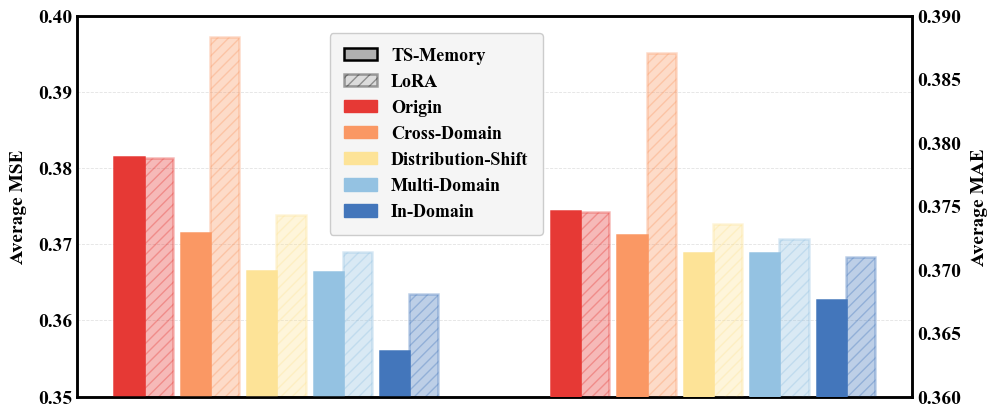
\includegraphics[width=\linewidth]{figures/tsmemory-vs-lora-cross-domain.png}
  \caption{TS-Memory vs. LoRA under different train-test domains. Full per-dataset results are provided in Table~\ref{tab:domain_split_lora_tsmemory}.}
  \Description{TS-Memory vs. LoRA under different train-test domains.}
  \label{tab:domain_split_lora_tsmemory_bar}
\end{figure}

\begin{figure}[!b]
  \centering
  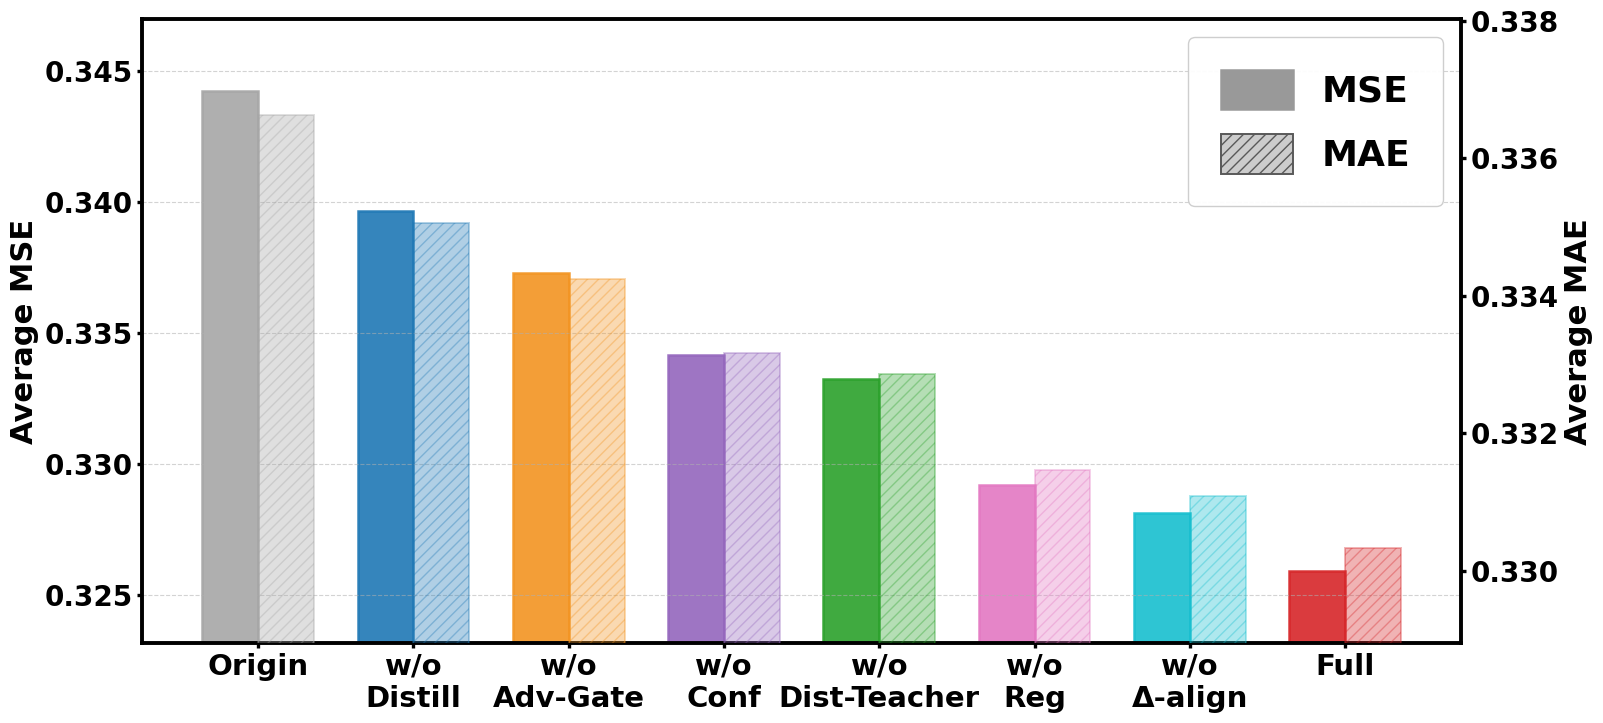
\includegraphics[width=\linewidth]{figures/abl_between_8groups.png}
  \caption{Ablation study of TS-Memory components.}
  \Description{Ablation study of TS-Memory components.}
  \label{fig:ablation_study}
\end{figure}


\noindent\textbf{Generalization under domain shift.}
\label{sec:transfer_domain_shift}
% Figure~\ref{fig:chronosbolt_kb_bar} assesses generalization by training PlugMem once with retrieval supervision from a source dataset and testing directly on a distinct target dataset (ChronosBolt backbone frozen). We consider five settings: \textit{Origin} (zero-shot ChronosBolt), \textit{Cross-Domain} (Weather $\rightarrow$ ETT), \textit{Distribution-Shift} (paired ETT transfer, e.g., ETTh1 $\leftrightarrow$ ETTh2), \textit{Multi-Domain} (pooled ETT knowledge base), and \textit{In-Domain} (target-specific supervision). Results show TS-Memory degrades gracefully under domain mismatch: cross-domain supervision from the unrelated Weather dataset still reduces average MSE by 2.7\%, verifying the learned memory captures transferable temporal patterns beyond dataset-specific traits. More related sources yield stronger, stabler gains: distribution-shift transfer achieves 3.5\% MSE reduction, while multi-domain transfer improves MSE by 4.0\% via diverse but related temporal dynamics. In-domain supervision performs best (6.8\% lower MSE, 1.9\% lower MAE on average), showing retrieval knowledge base-target distribution alignment amplifies benefits. These findings confirm TS-Memory gains scale smoothly with source-target similarity (no abrupt failure under mismatch). Conversely, LoRA shows limited cross-domain transfer and may underperform the frozen backbone on cross-domain data (Appendix~\ref{appx:complete_results}, Table~\ref{tab:lora_transfer_results}).
Figure~\ref{tab:domain_split_lora_tsmemory_bar} evaluates our method under domain shift on the ChronosBolt backbone. 
Table~\ref{tab:setting_test_relation} summarizes the train$\rightarrow
$test domain relations, where \textit{train} denotes the domain used to construct offline retrieval supervision and \textit{test} the target domain for evaluation.
% Figure~\ref{tab:domain_split_lora_tsmemory_bar} evaluates transfer under domain shift on the ChronosBolt backbone, with train$\rightarrow$test dataset relations summarized in Table~\ref{tab:setting_test_relation}. 
Even with mismatched supervision, TS-Memory provides non-trivial gains: cross-domain training reduces average MSE by 2.7\%, while more related transfer settings yield larger and more stable improvements, reaching 3.5\% MSE reduction under distribution-shift transfer and 4.0\% under multi-domain transfer. In-domain supervision performs best, achieving 6.8\% lower MSE and 1.9\% lower MAE on average, confirming that retrieval supervision is most effective when the knowledge base aligns with the target distribution. This smooth scaling with alignment suggests that TS-Memory does not rely on brittle dataset-specific shortcuts, but instead distills transferable temporal motifs. Meanwhile, LoRA exhibits weaker cross-domain robustness and can underperform the frozen backbone under domain mismatch. 





\subsection{Model Analysis}
\label{sec:model_analysis}

\noindent\textbf{Ablation study.}
\label{sec:model_analysis_ablation}
Figure~\ref{fig:ablation_study} reports component ablations averaged across datasets and horizons, where the full TS-Memory achieves the best overall performance (5.3\% lower MSE and 1.9\% lower MAE compared to the frozen backbone). When retrieval distillation is removed, the gains largely vanish, indicating that the offline retrieval teacher is the primary source of transferable corrective signal. Moreover, disabling either the advantage gate or the confidence-aware weighting consistently degrades performance, suggesting that \textit{selective} and \textit{confidence-conditioned} distillation is crucial: it filters unreliable retrieval targets and prevents negative transfer when retrieved futures are noisy or mismatched. Finally, auxiliary stability terms (e.g., Reg and $\Delta$-align) yield modest yet consistent improvements, primarily by stabilizing training and discouraging over-correction so that the learned memory behaves as a conservative correction module on top of the strong frozen prior.

% Figure~\ref{fig:ablation_study} presents component ablation results averaged across all datasets and horizons. The full TS-Memory achieves optimal overall performance, reducing MSE by 5.3\% and MAE by 1.9\% vs. the frozen backbone. Removing retrieval distillation drastically diminishes gains, confirming the offline retrieval teacher is the key driver of improvement. Disabling either the advantage gate or confidence-aware weighting further degrades performance, demonstrating that selective, confidence-conditioned distillation is critical to avoid negative transfer from imperfect retrieval targets. Finally, auxiliary stability terms (e.g., regularization, delta alignment) yield modest yet consistent benefits, primarily enhancing training stability and preventing over-correction.

% \noindent\textbf{Effect of retrieval knowledge base.}
% Figure~\ref{fig:chronosbolt_kb_bar} varies only the knowledge base used to build the offline retrieval teacher while keeping the frozen backbone, retrieval hyperparameters, and PlugMem training recipe unchanged.
% We fix ChronosBolt as the backbone and report average MSE/MAE over the four ETT benchmarks.
% Even cross-domain supervision remains beneficial, reducing average MSE by about 2.7\%.
% Using more closely related sources (distribution-shift or multi-domain knowledge bases) yields stronger and more stable gains (about 4.0\% MSE reduction), while in-domain supervision performs best with about 6.8\% lower MSE and 1.9\% lower MAE on average.
% These findings highlight that TS-Memory benefits scale with the alignment between the retrieval knowledge base and the target distribution.

\noindent\textbf{Scaling PlugMem capacity.}
\label{sec:model_analysis_scaling_capacity}
Figure~\ref{fig:Scaling Analysis of PlugMem} studies the effect of PlugMem capacity under a fixed training recipe and frozen backbone, focusing on long-horizon forecasting. Even a small PlugMem recovers most of the gain over the frozen TSFM, suggesting that the retrieval teacher mainly provides low-complexity correction patterns rather than requiring large task-specific parameterization. As capacity increases beyond a moderate size, improvements saturate and can slightly regress on some datasets, indicating over-correction or idiosyncratic artifacts from the teacher. Overall, a moderately sized PlugMem offers the best accuracy–efficiency trade-off for plug-and-play deployment. Accordingly, we design three PlugMem variants of different sizes (see Appendix~\ref{appx:complete_results}, Table~\ref{tab:mem-size}).

\begin{figure}[!t]
  \centering
  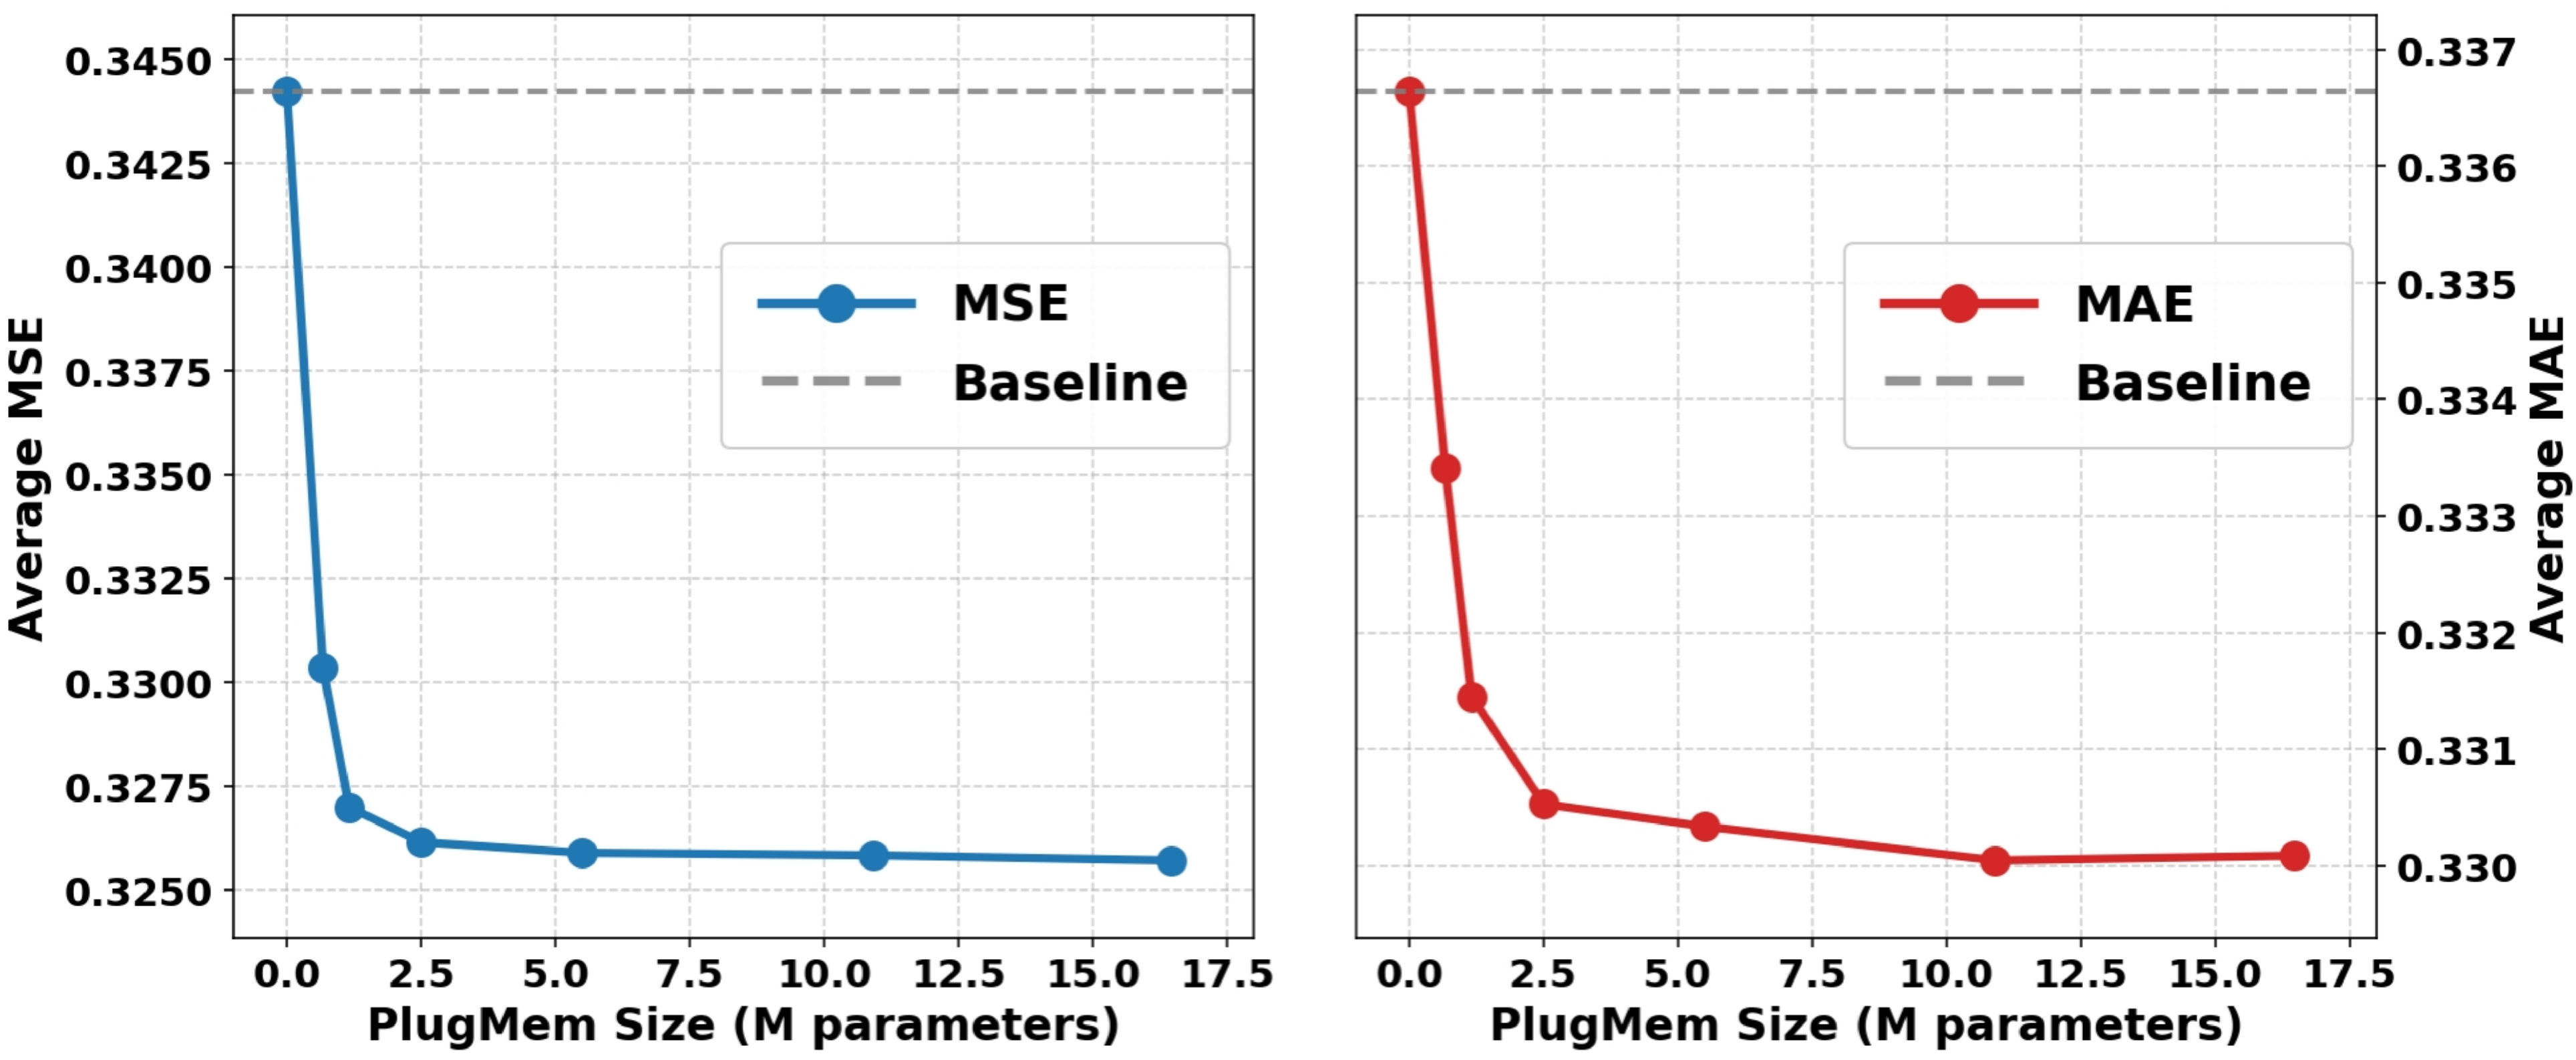
\includegraphics[width=\linewidth]{figures/plugmem_performance.png}

  \caption{Scaling Analysis of PlugMem Capacity. }
  \Description{Scaling analysis of PlugMem for long-term forecasting.}
  \label{fig:Scaling Analysis of PlugMem}

\end{figure}

% \begin{figure}[!htpb]
%     \centering
%     \begin{minipage}[t]{0.23\textwidth}
%         \centering
%         \includegraphics[width=\linewidth,height=3.2cm,keepaspectratio]{figures/plugmem_performance_mse.png}
%     \end{minipage}\hfill
%     \begin{minipage}[t]{0.23\textwidth}
%         \centering
%         \includegraphics[width=\linewidth,height=3.2cm,keepaspectratio]{figures/plugmem_performance_mae.png}
%     \end{minipage}

%     \caption{Scaling Analysis of PlugMem Capacity.}
%     \Description{Scaling analysis of PlugMem for long-term forecasting.}
%     \label{fig:Scaling Analysis of PlugMem}
% \end{figure}


% \input{tables/PlugMem Size-simple}
\begin{figure}[!b]
  \centering

  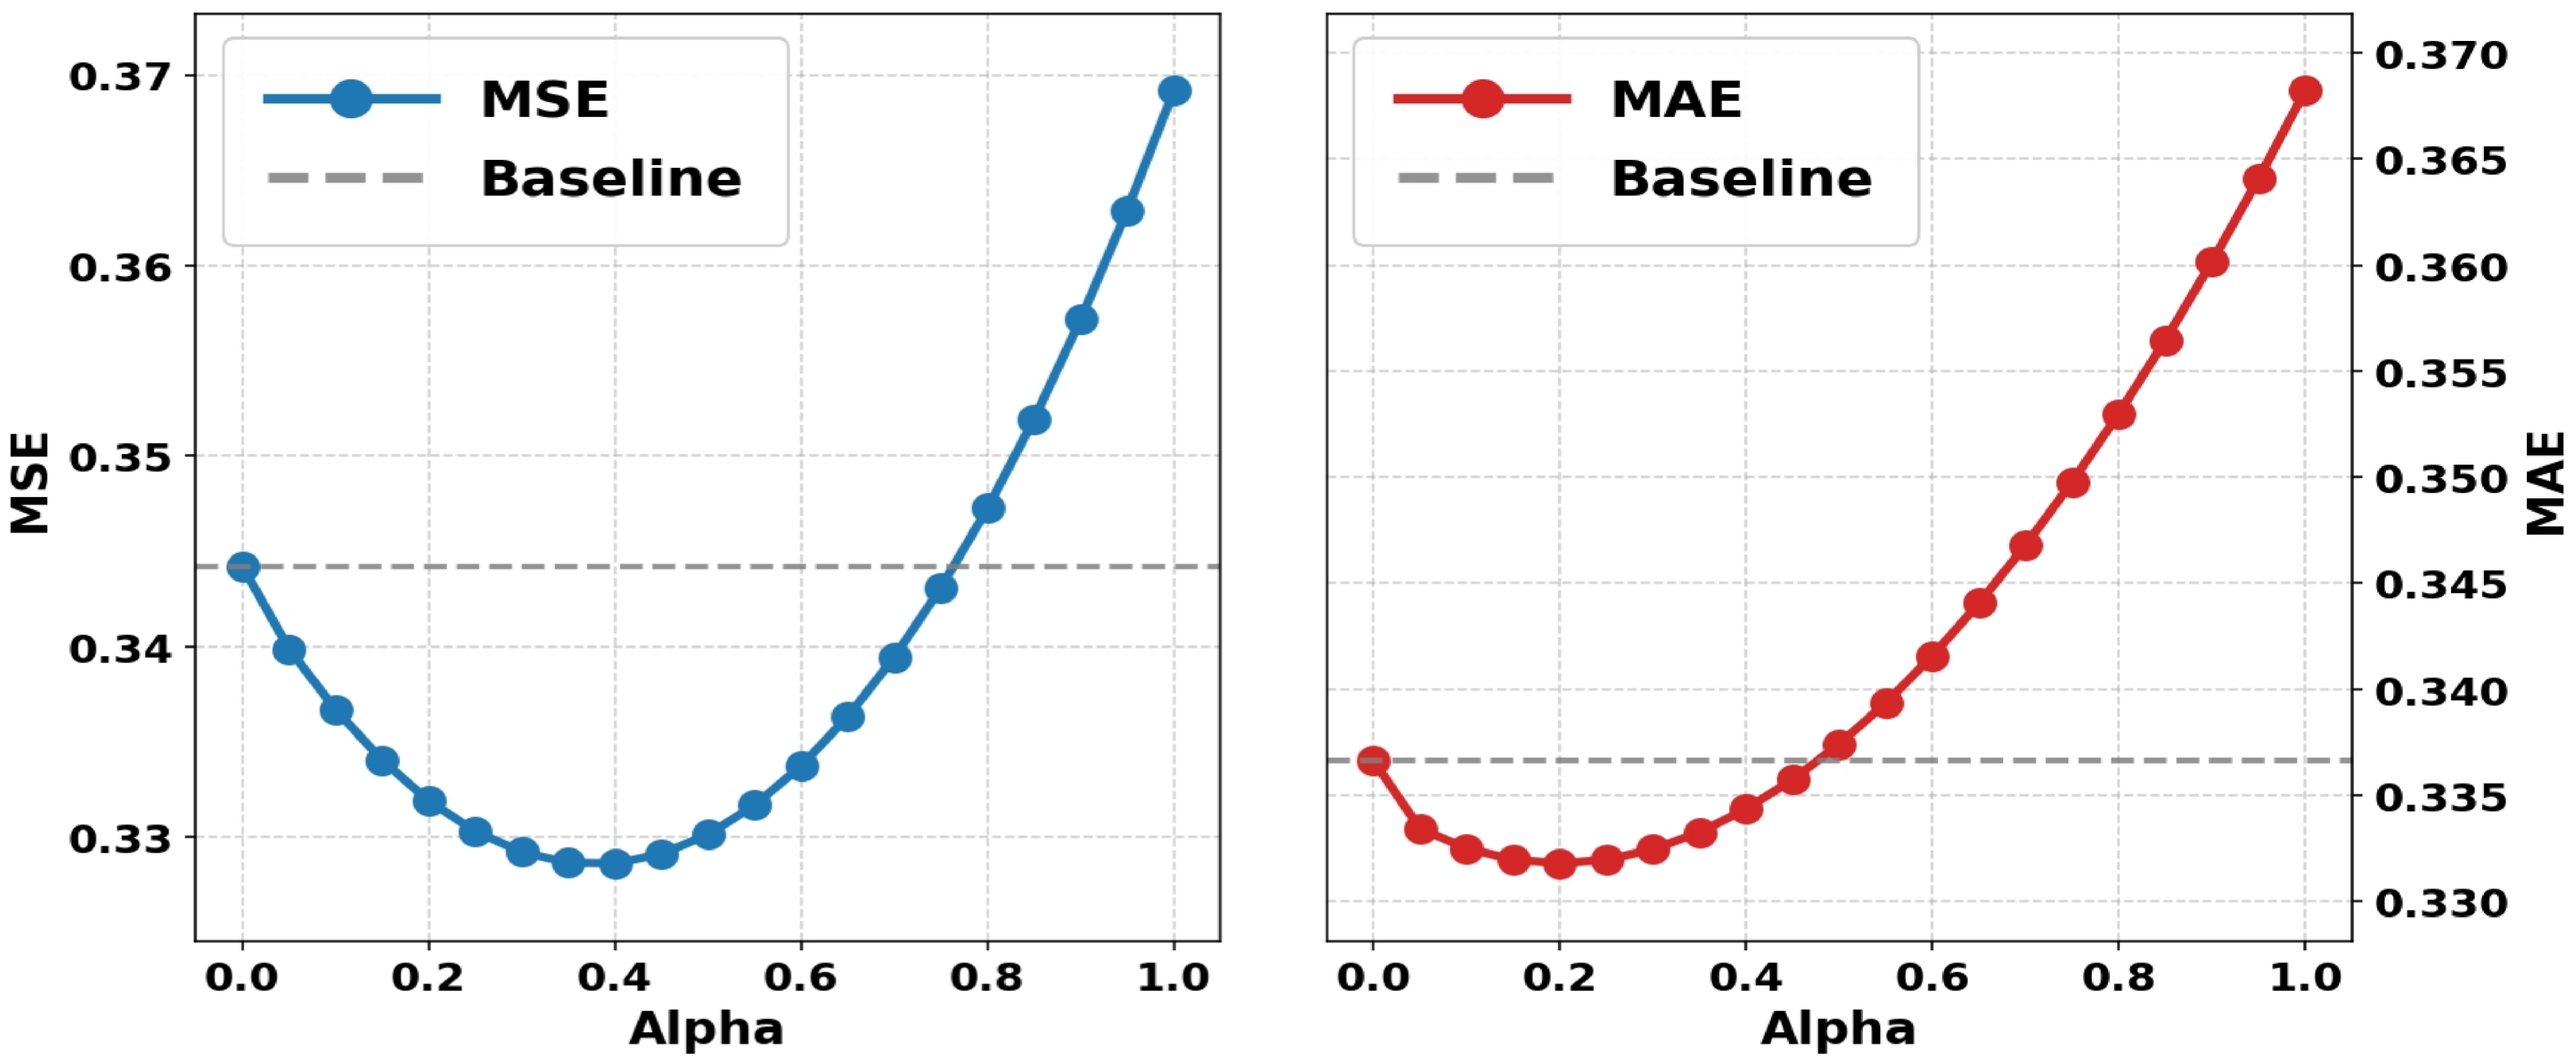
\includegraphics[width=\linewidth]{figures/alpha_ALL8_avg.png}

  \caption{Sensitivity Analysis of the Fusion Weight $\alpha$.}
  \Description{Sensitivity analysis of $\alpha$ for long-term forecasting.}
  \label{fig:sensitivity_analysis}
\end{figure}

\noindent\textbf{Sensitivity to the fusion weight.}
\label{sec:model_analysis_sensitivity_alpha}
% Figure~\ref{fig:sensitivity_analysis} analyzes the weight $\alpha$ for fusing backbone and PlugMem quantile forecasts. Performance improves with $\alpha$ increasing from 0, showing the memory branch provides complementary corrections (not redundant predictions). However, excessively large $\alpha$ degrades MSE/MAE, as over-reliance on memory overrides strong backbone priors and amplifies residual bias. Notably, the curve has a clear optimum and remains flat near it, enabling stable, lightweight validation-based tuning.
Figure~\ref {fig:sensitivity_analysis} analyzes the fusion weight $\alpha$ for combining backbone and PlugMem quantile forecasts. Performance improves as $\alpha$ increases from 0, confirming that the memory branch provides complementary corrections rather than redundant predictions. However, excessively large $\alpha$ degrades MSE/MAE, as over-reliance on memory overrides the strong priors learned by the backbone and amplifies residual bias; in the extreme case of $\alpha=1$, the backbone is discarded entirely in favor of PlugMem alone. Notably, the curve exhibits an optimum and remains flat near it, enabling stable, lightweight validation-based tuning.
% Figure~\ref {fig:sensitivity_analysis} analyzes the fusion weight $\alpha$ for combining backbone and PlugMem quantile forecasts. Performance improves as $\alpha$ increases from 0, confirming that the memory branch provides complementary corrections rather than redundant predictions. However, excessively large $\alpha$ degrades MSE/MAE, as over-reliance on memory overrides strong backbone priors and amplifies residual bias; in particular, $\alpha=1$ discards the backbone entirely and relies solely on PlugMem. Notably, the curve exhibits a clear optimum and remains flat near it, enabling stable, lightweight validation-based tuning.



% \begin{figure}[!htpb]
%     \centering
%     \begin{minipage}[t]{0.23\textwidth}
%         \centering
%         \includegraphics[width=\linewidth,height=3.2cm,keepaspectratio]{figures/alpha_ALL8_avg_mse.png}
%     \end{minipage}\hfill
%     \begin{minipage}[t]{0.23\textwidth}
%         \centering
%         \includegraphics[width=\linewidth,height=3.2cm,keepaspectratio]{figures/alpha_ALL8_avg_mae.png}
%     \end{minipage}

%     \caption{Sensitivity Analysis of the Fusion Weight $\alpha$.}
%     \Description{Sensitivity analysis of $\alpha$ for long-term forecasting.}
%     \label{fig:sensitivity_analysis}
% \end{figure}

% \noindent\textbf{Qualitative visualizations.}
% Figure~\ref{fig:qualitative_visualization} presents representative cases highlighting behavioral differences among methods. In (a), the frozen backbone and several baselines remain nearly flat after the forecast start (dashed line), failing to track the target's subsequent level shift, whereas TS-Memory produces a clear corrective trend better aligned with the ground truth—consistent with learning compact bias corrections from retrieval distillation. In (b), TS-RAG exhibits noticeable long-horizon drift and LoRA/RAFT introduce phase or smoothness artifacts, while TS-Memory stays closer to the ground-truth trajectory with reduced accumulated error, demonstrating that distilling retrieval \textit{offline} into a memory module preserves adaptability without online retrieval instability. In (c,d), probabilistic forecast comparisons illustrate why selective, confidence-aware training matters: PlugMem alone can become overly aggressive (mis-centered median and excessively wide or oscillatory PI), while the frozen backbone tends to be conservative but biased; TS-Memory balances both, yielding a well-calibrated PI width and better-centered median. Overall, these plots corroborate the ablation findings: advantage-gated, confidence-weighted distillation enables TS-Memory to absorb useful retrieval signals while suppressing unreliable teacher artifacts, producing a robust correction mechanism rather than a fragile replacement predictor.

\noindent\textbf{Gate statistics.}
Table~\ref{tab:gate_stats} summarizes how the advantage gate behaves during memory distillation. 
Here, $\chi_t{=}1$ indicates that the retrieval teacher outperforms the frozen backbone on a training window, $\omega_t$ is the confidence-weighted gate coefficient, and Adv. Margin measures the teacher's improvement over the backbone. 
Across all eight datasets, the teacher outperforms the backbone on $83.5\%$ of training windows, but the gate is not always-on. 
Activation and $\omega_t$ are lower on well-calibrated benchmarks such as Electricity and Traffic, while activation is much higher on shifting domains such as Weather and Exchange. 
This indicates that the gate acts as a domain-adaptive filter, selectively distilling useful retrieval signals while suppressing weak or uncertain teacher corrections.

\begin{table}[t]
\centering
\small
\caption{Gate activation statistics during confidence-gated memory distillation.}
\label{tab:gate_stats}
\begin{tabular*}{\linewidth}{@{\extracolsep{\fill}}lcccc}
\toprule
Dataset & Act. $(\chi_t{=}1)$ & Mean $\omega_t$ & Mean Conf. & Adv. Margin \\
\midrule
ETT Avg     & $87.7\%$ & 0.479 & 0.562 & 0.173 \\
Weather     & $96.7\%$ & 0.680 & 0.701 & 0.245 \\
Traffic     & $68.1\%$ & 0.067 & 0.100 & 0.025 \\
Electricity & $50.8\%$ & 0.062 & 0.113 & 0.013 \\
Exchange    & $99.4\%$ & 0.102 & 0.102 & 0.184 \\
\bottomrule
\end{tabular*}
\end{table}


\begin{figure}[!b]
  \centering
  \includegraphics[width=\linewidth]{figures/TS-Memory-vision.png}

  \caption{Qualitative visualizations comparing TS-Memory with the frozen backbone and adaptation baselines.}
  \Description{Qualitative Visualization.}
  \label{fig:qualitative_visualization}

\end{figure}
\noindent\textbf{Qualitative visualizations.}
Figure~\ref{fig:qualitative_visualization} presents representative cases highlighting behavioral differences among methods. In (a), the frozen backbone and several baselines remain nearly flat after the forecast start (dashed line), failing to track the target's subsequent level shift, whereas TS-Memory produces a clear corrective trend that is better aligned with the ground truth, consistent with learning compact bias corrections from retrieval distillation. In (b), TS-RAG exhibits noticeable long-horizon drift, and LoRA/RAFT introduce phase or smoothness artifacts, while TS-Memory stays closer to the ground-truth trajectory with reduced accumulated error, demonstrating that distilling retrieval offline into a memory module preserves adaptability without the instability inherent in online retrieval. In (c,d), probabilistic forecast comparisons illustrate why selective, confidence-aware training matters: PlugMem alone can become overly aggressive, producing a mis-centered median and excessively wide or oscillatory prediction intervals, while the frozen backbone tends to be conservative but biased; TS-Memory balances both, yielding well-calibrated interval width and a more accurately centered median. Overall, these plots corroborate the ablation findings: advantage-gated, confidence-weighted distillation enables TS-Memory to absorb useful retrieval signals while suppressing unreliable teacher artifacts, producing a robust correction mechanism rather than a fragile replacement predictor.









